\documentclass[12pt, spanish]{article}
\usepackage[spanish]{babel}
\selectlanguage{spanish}
\usepackage{natbib}
\usepackage{url}
\usepackage[utf8x]{inputenc}
\usepackage{graphicx}
\graphicspath{{images/}}
\usepackage{parskip}
\usepackage{fancyhdr}
\usepackage{vmargin}
\usepackage{multirow}
\usepackage{float}
\usepackage{chngpage}

\usepackage{subcaption}

\usepackage{hyperref}
\usepackage[
    type={CC},
    modifier={by-nc-sa},
    version={4.0},
]{doclicense}

\hypersetup{
    colorlinks=true,
    linkcolor=blue,
    filecolor=magenta,      
    urlcolor=cyan,
}

% para codigo
\usepackage{listings}
\usepackage{xcolor}



%% configuración de listings

\definecolor{listing-background}{HTML}{F7F7F7}
\definecolor{listing-rule}{HTML}{B3B2B3}
\definecolor{listing-numbers}{HTML}{B3B2B3}
\definecolor{listing-text-color}{HTML}{000000}
\definecolor{listing-keyword}{HTML}{435489}
\definecolor{listing-identifier}{HTML}{435489}
\definecolor{listing-string}{HTML}{00999A}
\definecolor{listing-comment}{HTML}{8E8E8E}
\definecolor{listing-javadoc-comment}{HTML}{006CA9}

\lstdefinestyle{eisvogel_listing_style}{
  language         = c++,
%$if(listings-disable-line-numbers)$
%  xleftmargin      = 0.6em,
%  framexleftmargin = 0.4em,
%$else$
  numbers          = left,
  xleftmargin      = 0em,
 framexleftmargin = 0em,
%$endif$
  backgroundcolor  = \color{listing-background},
  basicstyle       = \color{listing-text-color}\small\ttfamily{}\linespread{1.15}, % print whole listing small
  breaklines       = true,
  frame            = single,
  framesep         = 0.19em,
  rulecolor        = \color{listing-rule},
  frameround       = ffff,
  tabsize          = 4,
  numberstyle      = \color{listing-numbers},
  aboveskip        = 1.0em,
  belowskip        = 0.1em,
  abovecaptionskip = 0em,
  belowcaptionskip = 1.0em,
  keywordstyle     = \color{listing-keyword}\bfseries,
  classoffset      = 0,
  sensitive        = true,
  identifierstyle  = \color{listing-identifier},
  commentstyle     = \color{listing-comment},
  morecomment      = [s][\color{listing-javadoc-comment}]{/**}{*/},
  stringstyle      = \color{listing-string},
  showstringspaces = false,
  escapeinside     = {/*@}{@*/}, % Allow LaTeX inside these special comments
  literate         =
  {á}{{\'a}}1 {é}{{\'e}}1 {í}{{\'i}}1 {ó}{{\'o}}1 {ú}{{\'u}}1
  {Á}{{\'A}}1 {É}{{\'E}}1 {Í}{{\'I}}1 {Ó}{{\'O}}1 {Ú}{{\'U}}1
  {à}{{\`a}}1 {è}{{\'e}}1 {ì}{{\`i}}1 {ò}{{\`o}}1 {ù}{{\`u}}1
  {À}{{\`A}}1 {È}{{\'E}}1 {Ì}{{\`I}}1 {Ò}{{\`O}}1 {Ù}{{\`U}}1
  {ä}{{\"a}}1 {ë}{{\"e}}1 {ï}{{\"i}}1 {ö}{{\"o}}1 {ü}{{\"u}}1
  {Ä}{{\"A}}1 {Ë}{{\"E}}1 {Ï}{{\"I}}1 {Ö}{{\"O}}1 {Ü}{{\"U}}1
  {â}{{\^a}}1 {ê}{{\^e}}1 {î}{{\^i}}1 {ô}{{\^o}}1 {û}{{\^u}}1
  {Â}{{\^A}}1 {Ê}{{\^E}}1 {Î}{{\^I}}1 {Ô}{{\^O}}1 {Û}{{\^U}}1
  {œ}{{\oe}}1 {Œ}{{\OE}}1 {æ}{{\ae}}1 {Æ}{{\AE}}1 {ß}{{\ss}}1
  {ç}{{\c c}}1 {Ç}{{\c C}}1 {ø}{{\o}}1 {å}{{\r a}}1 {Å}{{\r A}}1
  {€}{{\EUR}}1 {£}{{\pounds}}1 {«}{{\guillemotleft}}1
  {»}{{\guillemotright}}1 {ñ}{{\~n}}1 {Ñ}{{\~N}}1 {¿}{{?`}}1
  {…}{{\ldots}}1 {≥}{{>=}}1 {≤}{{<=}}1 {„}{{\glqq}}1 {“}{{\grqq}}1
  {”}{{''}}1
}
\lstset{style=eisvogel_listing_style}


\usepackage[default]{sourcesanspro}

\setmarginsrb{2 cm}{1 cm}{2 cm}{2 cm}{1 cm}{1.5 cm}{1 cm}{1.5 cm}

\title{Práctica 3:\\
PAR - Búsquedas por Trayectorias  \hspace{0.05cm} }                           
\author{Antonio David Villegas Yeguas}                             
\date{\today}                                           

\renewcommand*\contentsname{hola}

\makeatletter
\let\thetitle\@title
\let\theauthor\@author
\let\thedate\@date
\makeatother

\pagestyle{fancy}
\fancyhf{}
\rhead{\theauthor}
\lhead{\thetitle}
\cfoot{\thepage}

\begin{document}

%%%%%%%%%%%%%%%%%%%%%%%%%%%%%%%%%%%%%%%%%%%%%%%%%%%%%%%%%%%%%%%%%%%%%%%%%%%%%%%%%%%%%%%%%

\begin{titlepage}
    \centering
    \vspace*{0.3 cm}
    
\includegraphics[scale = 0.50]{ugr.png}\\[0.7 cm]
    %\textsc{\LARGE Universidad de Granada}\\[2.0 cm]   
    \textsc{\large 3º CSI 2019/20 - Grupo 1}\\[0.5 cm]            
    \textsc{\large Grado en Ingeniería Informática}\\[0.5 cm]              
    \rule{\linewidth}{0.2 mm} \\[0.2 cm]
    { \huge \bfseries \thetitle}\\
    \rule{\linewidth}{0.2 mm} \\[1 cm]
    
    \begin{minipage}{0.4\textwidth}
        \begin{flushleft} \large
            \emph{Autor:}\\
            \theauthor\\ 
			 \emph{DNI:}\\
            77021623-M
            \end{flushleft}
            \end{minipage}~
            \begin{minipage}{0.4\textwidth}
            \begin{flushright} \large
            \emph{Asignatura: \\
            Metaheurísticas}   \\     
            \emph{Correo:}\\
            advy99@correo.ugr.es           
        \end{flushright}
    \end{minipage}\\[0.5cm]
  
    {\large \thedate}\\[0.5cm]
    {\url{https://github.com/advy99/MH/}}
    {\doclicenseThis}
 	
    \vfill
    
\end{titlepage}

%%%%%%%%%%%%%%%%%%%%%%%%%%%%%%%%%%%%%%%%%%%%%%%%%%%%%%%%%%%%%%%%%%%%%%%%%%%%%%%%%%%%%%%%%

\tableofcontents
\pagebreak

%%%%%%%%%%%%%%%%%%%%%%%%%%%%%%%%%%%%%%%%%%%%%%%%%%%%%%%%%%%%%%%%%%%%%%%%%%%%%%%%%%%%%%%%%


\section{Descripción del problema de la asignación con restricciones.}

El problema de la asignación con restricciones consiste en una generalización del problema de agrupamiento clásico, bastante común en \textit{Machine Learning}.

El problema del agrupamiento clásico es un problema en el que se recibe como entrada las características de un conjunto de elementos y el número de agrupaciones a realizar, para resolver el problema tendremos como objetivo realizar dichas agrupaciones de los distintos elementos con el fin de organizarlos acorde a las características dadas. Llamaremos a estas agrupaciones \textit{Clusters}.

Como extensión a este problema, nosotros trabajaremos sobre el problema de asignación con restricciones (de ahora en adelante PAR). PAR se basa en el problema del agrupamiento clásico, pero añadiendo al problema restricciones entre los propios elementos, es decir, las distintas parejas que podemos formar con los datos tendrán asociadas restricciones de dos tipos:

\begin{itemize}
	\item{Must-Link (ML): Dados dos datos $D_1$ y $D_2$, si estos datos tienen asociada una restricción ML deberán tener asignado el mismo cluster.}
	\item{Cannot-Link (CL): Dados dos datos $D_1$ y $D_2$, si estos datos tienen asociada una restricción CL deberán tener asignado distinto cluster.}
\end{itemize}

Nosotros trataremos estas restricciones como restricciones débiles, es decir, permitiremos que se incumplan pero penalizándolas, por lo tanto, el objetivo para resolver el PAR es minimizar la distancia de los elementos que conforman los distintos clusters, así como asegurarnos que no se incumple ninguna restricción.

Otra restricción fuerte del problema es que todos los clusters tienen que tener al menos un elemento.

Para comprobar que la distancia entre los elementos de los distintos clusters es mínima, tendremos las siguientes características asociadas a un cluster:

\begin{itemize}
	\item{Centroide: Valor promedio de los datos que conforman el cluster. Con este elementos obtendremos la representación del elemento central del cluster.}
	\item{Distancia media intra-cluster: Con este elemento mediremos como de disperso está nuestro cluster, es decir, si los elementos de un cluster están cercanos entre si.}
\end{itemize}

Además también contaremos con distintas características del PAR:

\begin{itemize}
	\item{Desviación general: Será la media de las desviaciones intra-cluster de los distintos clusters que conforman el PAR. Uno de nuestros objetivos será que este valor sea mínimo.}
	\item{\textit{Infeasibility}: Esta característica nos permitirá conocer cuantas restricciones se están incumpliendo en una posible solución del PAR. Otro de nuestros objetivos será que este valor sea mínimo.}
\end{itemize}

\newpage

\section{Descripción de la implementación común y representación del problema para su resolución.}

Para el desarrollo e implementación del programa que resolverá el PAR he decidido usar C++ como lenguaje de programación.

Para la representación del problema he decidido construir dos clases en C++, la clase PAR y la clase Cluster.



\subsection{Clase PAR:}


Esta clase contará con los siguientes atributos:

\begin{itemize}
	\item {Matriz que almacenará valores reales, donde estarán las características de los datos.}
	\item {Vector de objetos tipo Cluster con el que representaremos las agrupaciones a conseguir.}
	\item {Diccionario con las restricciones entre los distintos datos.}
	\item {Desviación general del problema.}
	\item {Mayor distancia entre dos los distintos datos del problema.}
	\item {\textit{Infeasibility} del problema}
\end{itemize}


\subsection{Clase Cluster:}

Con esta clase representaremos los elementos y operaciones internas de un cluster. Tendrá los siguientes atributos:

\begin{itemize}
	\item {Set que almacenará enteros, representando que elementos conforman dicho cluster.}
	\item {Vector de reales que representará el centroide.}
	\item {Valor real que representará la distancia intra-cluster de los elementos que lo conforman.}
	\item {Una referencia a la clase PAR asociada, con la que obtendremos los datos necesarios sin necesidad de duplicarlos.}
\end{itemize}

Es importante mencionar que la declaración de la clase Cluster se realiza dentro de la clase PAR, ya que no tiene sentido crear un cluster sin tener un problema asociado.


\newpage

\subsection{Representación:}

\subsubsection{Datos:}

Con respecto a la representación del problema, los datos son almacenados en una matriz de datos tipo \texttt{double}, cada fila representará un dato, y las columnas representarán las características de dicho dato.

\subsubsection{Restricciones:}

Las restricciones serán almacenadas en un diccionario, donde la clave será la pareja de datos afectada por la restricción y el valor será 1 si la restricción es ML o -1 si es CL. He decidido usar esta representación ya que nos permite almacenar la información de forma eficiente sin tener que almacenar los elementos que no tiene restricciones entre sí, nos permite acceder a los elementos de una forma más rápida que con una lista (aunque no tanto comparado con una matriz, pero gracias al operador \texttt{find} de la clase esto apenas se nota) y podemos recorrer las restricciones secuencialmente de una forma rápida gracias a los iteradores disponibles en la clase diccionario de C++.


Con esta representación de los datos y las restricciones, las distintas operaciones antes comentadas se pueden resolver de forma sencilla generalizando el número de generalizando el número de características, independientemente del problema.


\subsubsection{Solución:}

Para representar la solución he decido, como he comentado anteriormente, que la solución esté compuesta por un vector de objetos tipo cluster, a pesar de que esta representación no será valida para futuras prácticas, es mucho más sencillo y práctico trabajar con ella en la primera práctica, ya que al separar los distintos clusters en su propio objeto podemos realizar las operaciones que afecten a los clusters de forma mucho más rápida y permitiendo la factorización del problema, ya que por ejemplo, seremos capaces de recalcular el centroide de un cluster sin tener que tener en cuenta los demás, o separar los elementos.

La representación dada en clase (vector de enteros de tamaño N siendo N el número de datos, y cada posición del vector se le asocia un número, que será el cluster al que pertenece) es de gran utilidad en la práctica 2, por lo que tenemos una función que nos intercambiará entre estas soluciones, es decir, una función que dado un vector de clusters nos devolverá un vector de enteros con las asignaciones del argumento dado.

\begin{lstlisting}
//vector de ints en el que devolveremos la solución
vector_sol 

Para todo cluster i en el vector de clusters:
	Para todo elemento j en el cluster i:
		vector_sol[j] = i;
		
Devolver vector_sol

\end{lstlisting}


\subsubsection{Operaciones sobre los clusters:}

Los clusters tendrán principalmente dos funciones que podremos realizar:

\begin{itemize}
	\item {Calcular el centroide}
	\item {Calcular la distancia media intra-cluster}
\end{itemize}

Para calcular el centroide basta con recorrer los elementos que conforman ese cluster (disponibles dentro de la clase Cluster) y calcular el punto medio.

\begin{lstlisting}
Para i = 0 hasta el tamaño del centroide (numero de caracteristicas de un dato) :
	centroide[i]=0.0d
	
Para cada elemento i del cluster:
	Para cada carasterictica j del elemento i:
		centroide[j] += problema.datos[i][j];
		
Para cada caracteristica i del centroide:
	centroide[i] /= num_elementos_cluster 
	
	
\end{lstlisting}

Para calcular la distancia media intra-cluster calcularemos el centroide y tras eso la distancia de todos los elementos al centroide.


\begin{lstlisting}
calcular_centroide();
distancia_intra_cluster = 0
	
Para cada elemento i del cluster:
	Para cada carasterictica j del elemento i:
		distancia_intra_cluster += problema.datos[i][j];
		
Para cada caracteristica i del centroide:
	distancia_intra_cluster /= num_elementos_cluster 
	
	
\end{lstlisting}

\newpage

\subsubsection{Operaciones sobre PAR:}

Sobre el problema podremos aplicar las siguientes operaciones:

\begin{itemize}
	\item {Calcular la desviación general.}
	\item {Buscar el cluster en el que se encuentra cierto elemento.}
	\item {Calcular \textit{Infeasibility} del estado actual del PAR.}
	\item {Calcular la distancia entre dos puntos del problema.}
\end{itemize}

Para calcular la desviación general haremos la media de las distintas desviaciones intra-cluster.


\begin{lstlisting}
desviacion_general = 0
	
Para cada elemento i del vector de clusters:
	clusters[i].calcular_desviacion_intra_cluster()
	desviacion_general += cluster[i].desviacion_intra_cluster()
		
desviacion_general /= clusters.size()	
	
\end{lstlisting}

Para buscar un elemento N dado por parámetro en los distintos clusters simplemente recorreremos el vector de clusters usando el operador find de la clase set, al estar ordenados y ser únicos, esto hará que esta operación sea muy rápida.

\begin{lstlisting}
encontrado = false
encontrado_en_cluster = -1

Mientras !encontrado Y para cada elemento i del vector clusters
	Si clusters[i].elementos.find(N) != clusters[i].elementos.end()
		encontrado = true	
		encontrado_en_cluster = i
		
return encontrado_en_cluster
	
\end{lstlisting}


Para calcular  \textit{Infeasibility} del PAR simplemente recorreremos el diccionario de restricciones, si encontramos dos elementos en distinto cluster y son ML sumamos 1 al total, y si encontramos dos elementos en el mismo cluster y tienen la restricción de CL sumamos 1 al total.

Solo comprobaremos si en el diccionario, la pareja de datos el primer elemento es mayor que el segundo. Esto lo hacemos para evitar contar dos veces la misma restricción, por ejemplo, si tenemos la restricción 0 con 1: ML, también tenemos la 1 con 0: ML, así que solo comprobaremos la 1 con 0. A pesar de usar el diccionario he decidido duplicar de esta forma las restricciones ya que a veces necesitaremos acceder sin tener en cuenta el orden de los datos.

\newpage

\begin{lstlisting}
infac = 0

Para cada elemento i de  restricciones
	Si i.first.first > i.first.second
		Si existe una restricción entre i.first.first e i.first.second
			c1 = buscar_elemento(i.first.first)
			c1 = buscar_elemento(i.first.second)
			
			Si c1 == c2 Y i.second == -1
				infac++
			Si c1 != c2 Y i.second == 1
				infac++
		
		
return infac
	
	
\end{lstlisting}



 \textbf{Generador de solución inicial aleatoria.}
 
 Primero he desarrollado una función que nos genera una solución aleatoria que cumple con las restricciones fuertes (todos los clusters tienen al menos un elemento).
 
 \begin{lstlisting}
vaciar_clusters()

indices_aleatorios = {0...datos.size()}

indices_aleatorios = random_shuffle(indices)

contador = 0

// nos aseguramos que cada cluster tiene uno al menos
Para cada indice i desde 0 hasta clusters.size():
	clusters[i].insertar_elemento(indices_aleatorios[contador])
	contador++
	
Para contador < indices_aleatorios.size()
	clusters[EnteroAleatorio(0, clusters.size())].insertar_elemento(indices_aleatorios[contador])
	contador++
	

\end{lstlisting}
 


Tanto en PAR como en Cluster tendremos otras operaciones auxiliares relativas a los algoritmos de búsqueda o comparación, que explicaré más adelante.


\subsection{Calcular \textit{Infeasibility} parcial.}

Para hacer una factorización, además de poder calcular los atributos de los clusters de forma independiente sin necesidad de recalcular la de todos si no son modificados también necesitaremos una función que dado un cluster y un elemento nos calcula cuantas restricciones incumpliría si lo introducimos en dicho cluster.


\begin{lstlisting}
elemento: nos lo dan como argumento
cluster: nos lo dan como argumento

incumplidas = 0


Para todos los elementos i del cluster dado:
	Si i y elemento tienen una restricción Y dicha restricción == -1
		incumplidas++

Para los elementos j de los clusters != cluster:
	Si j y elemento tienen una restricción Y dicha restricción == 1
		incumplidas++



return incumplidas
	
	
\end{lstlisting}

\subsection{Función objetivo.}

En el caso del PAR nuestro objetivo será agrupar los datos en clusters incumpliendo el mínimo de restricciones.

Para cumplir la primera parte intentaremos que los datos estén lo menos dispersos con respecto a su centroide, por lo que intentaremos minimizar el total de las desviaciones intra-cluster, en resumen, \textbf{minimizar la desviación general}. 

Para la segunda parte, intentaremos minimizar el número de restricciones incumplidas penalizando las soluciones que más restricciones incumplan. Esta penalización se basará en sumar a la desviación general un valor entre 0 y la distancia más grande entre los datos del problema.

Esto lo conseguiremos con este factor, al que llamaremos $\lambda$:

$$ \lambda = \frac{D_{max}}{NumRestricciones} $$ 


De forma que si incumplimos todas las restricciones la solución la consideraremos mucho peor que otra con mayor desviación general pero menor restricciones incumplidas.

Nuestra función objetivo será:

$$ f = C + (\textit{Infeasibility} * \lambda) $$ 


\newpage

\section{Métodos de resolución del problema.}

\subsection{Algoritmo de Búsqueda Local.}

Este algoritmo se basa en partir de una solución inicial aleatoria, a partir de esa solución explorar una solución vecina, y si esta solución vecina es mejor que la actual, moverse a dicha solución.

Este algoritmo no nos asegurará obtener el optimo, solo nos garantiza obtener un mínimo local (puede que este mínimo local sea el optimo, pero no lo podemos asegurar).

El algoritmo solo cambiará una solución por otra mejor, por lo que el punto de inicio será muy importante.

Para desarrollar este algoritmo necesitamos varios componentes:
 
 
\subsubsection{Generador de vecinos}

En nuestro caso, construiremos el vecindario a partir de una solución, modificando un único elemento de cluster, siempre que no se queden clusters vacíos, es decir, si tenemos una solución S, generaremos un vecino $S_1$ eliminando un elemento de un cluster $i$ e insertandolo en otro cluster $j$, siempre que el cluster $i$ no se quede vacío y $i$ sea distinto a $j$.

El elemento a mover y el nuevo cluster lo escogeremos de forma aleatoria, como explicaré más adelante en el desarrollo del algoritmo completo.

 
\subsubsection{Función objetivo} 
 
Una vez tenemos una primera solución, necesitamos conocer como obtener el valor de la función objetivo asociada a esa función.

Cada vez que generemos un vecino recalcularemos su desviación general, por lo que calcular su función objetivo será:

\begin{lstlisting}
funcion_objetivo = get_desviacion_promedio + ( LAMBDA * calcular_infactibilidad() )
 \end{lstlisting}


Sin embargo, para reducir el tiempo de ejecución vamos a factorizar el cálculo de \textit{Infeasibility}, ya que dado un \textit{Infeasibility} de X, el valor para cualquier vecino será:

$$X - \textit{Infeasibility}\_cambios\_salida + \textit{Infeasibility}\_cambios\_entrada$$
 
 Al solo modificar un elemento por vecino, \textit{Infeasibility}\_cambios\_salida  es el número de restricciones que incumplía dicho elemento en el cluster antiguo y \textit{Infeasibility}\_cambios\_entrada es el número de restricciones que incumple el nuevo cluster.
 
 
 
\begin{lstlisting}
infact -= cumple_restricciones(elemento, antiguo_num_cluster)
infact += cumple_restricciones(elemento, nuevo_num_cluster)

funcion_objetivo = get_desviacion_promedio + ( LAMBDA * calcular_infactibilidad() )
 \end{lstlisting}

\subsubsection{Criterio de aceptación.}

Se aceptará un vecino si su función objetivo es menor que la de la solución actual, es decir, seguiremos una estrategia primero el mejor, en cuanto tengamos un mejor candidato nos movemos a el, en lugar de generar todo el vecindario y quedarnos con el mejor del vecindario.

Finalizaremos la búsqueda si no encontramos mejor vecino en todo el vecindario.

\subsubsection{Exploración del entorno.}

La exploración del entorno se realizará de forma aleatoria, cada iteración (no evaluación) reordenaremos de forma aleatoria los indices con los que recorreremos los elementos y los indices con los que recorreremos los clusters. Cada elemento lo probaremos con los distintos clusters (a excepción del propio), por lo que iremos generando los vecinos de cada elemento sin llegar a generar el vecindario completo, solo generamos vecindario hasta que encontramos un mejor vecino. Lo veremos más adelante en el algoritmo.

\subsubsection{Desarrollo del algoritmo.}

El algoritmo de búsqueda local se basará en generar una solución aleatoria, a partir de esa solución aleatoria generar vecinos, evaluarlos hasta que encuentre un mejor vecino, en cuanto encuentre un mejor vecino moverse a este, y parar en caso de que en todo el vecindario no encuentre un mejor vecino o se llegue al límite de evaluaciones, en nuestro caso 100.000.

\newpage

Con las distintas operaciones podemos codificar el algoritmo de la siguiente forma:

{\small
\begin{lstlisting}
generar_solucion_aleatoria()
calcular_desviacion_general()

LAMBDA = mayor_distancia / restricciones.size()
evaluaciones = 0
encontrado_mejor = false
indices = {0..datos.size()}
indices_clusters = {0..clusters.size()}
infac = calcular_infactibilidad()
infac_vecino = infac
f_objetivo = get_desviacion_general() + (infac * LAMBDA)
f_objetivo_vecino = 0

do:
	encontrado_mejor = false
	reordenar_aleatoriamente(indices)
	reordenar_aleatoriamente(indices_clusters)
	
	Para cada elemento i de indices Y !encontrado_mejor
		Para cada elemento j del indices_clusters Y !encontrado_mejor
			antiguo_cluster = buscar_elemento(i)
			Si antiguo_cluster != j Y clusters[antiguo_cluster].size() - 1 > 0
				clusters[antiguo_cluster].eliminar_elemento(i)
				infac_vecino -= incumple_restricciones(i, antiguo_cluster)
				infac_vecino += incumple_restricciones(i, j)
				clusters[j].añadir_elemento(i)
				calcular_desviacion_general()
				
				f_objetivo_vecino = get_desviacion_general() + (infac_vecino * LAMBDA)
				evaluaciones++				
				
				Si f_objetivo_vecino < f_objetivo
					f_objetivo = f_objetivo_vecino
					infac = infac_vecino
					encontrado_mejor = true
				Si NO
					clusters[j].eliminar_elemento(i)
					clusters[antiguo_cluster].añadir_elemento(i)
					infact_vecino = infac

while evaluaciones < TOPE_BL Y encontrado_mejor
 \end{lstlisting}
 }
 
 
Como consideraciones a este algoritmo, vemos como por el operador de vecino es posible que nos estanquemos en mínimos locales de los que no seamos capaces de salir, siendo este el principal problema del algoritmo de búsqueda local.

También mencionar que el escoger la función objetivo puede hacer variar la solución de una forma bastante importante dependiendo del peso que le demos a incumplir las restricciones, como veremos más adelante en los análisis de los resultados y experimentos, ya que de la función objetivo dependerá la penalización por incumplir restricciones por lo que modificando esta función podremos escoger entre mejorar la desviación general o no permitir que se incumplan restricciones.


\subsection{Algoritmo de Búsqueda Multiarranque Básica (BMB).}

Este algoritmo se basa en ejecutar múltiples veces el algoritmo de búsqueda local sobre soluciones generadas de forma aleatoria y quedarnos con la mejor solución que encontremos. De esta forma paliamos levemente el principal problema de la búsqueda local, que la exploración es nula y la solución obtenida depende exclusivamente de si el mínimo más cercano al punto de arranque es un buen mínimo. 

\begin{lstlisting}
Devuelve: vector de cluster (solución) y valoración de la solución - Recibe: num_sols - número de soluciones a obtener por BL y num_ite - iteraciones de cada BL

	//
	mejor = pareja<NULL, infinito>
	Para i = 0 hasta num_sols:
		solucion = generar_solucion_aleatoria();
		sol_i = algoritmo_BL(solucion, num_ite);
		
		Si sol_i.second < mejor.second
			mejor = sol_i
		
	// cargamos la mejor en los clusters y la devolvemos
	clusters = mejor.first;		
	return mejor; 

\end{lstlisting} 

Este algoritmo como vemos no es de gran complejidad, más adelante veremos como se comporta.

\subsection{Algoritmo de Enfriamiento Simulado (ES).}

Este algoritmo se trata de una modificación de la búsqueda local para añadirle diversidad. La idea de este algoritmo es diversificar al inicio de la ejecución del algoritmo y según avance el algoritmo y nos quede menos tiempo (iteraciones en nuestro caso) explotaremos la solución.

Para añadir esta diversidad e intentar conseguir el equilibrio exploración/explotación añadiremos un nuevo componente, la temperatura. Con este nuevo componente simularemos el enfriamiento de esta temperatura a lo largo del algoritmo, y en su ejecución aceptaremos un cambio de una solución a su vecino si el vecino es mejor o por un criterio dependiendo de la temperatura que explicaré más adelante, de forma que a mayor temperatura mayor será la probabilidad de aceptar un vecino aunque este sea peor. De esta forma el objetivo del algoritmo es comenzar con una temperatura alta de forma que se aceptarán soluciones peores lo que permitirá salir de mínimos locales, y según avance la ejecución la temperatura disminuirá, simulando el enfriamiento de esta, de forma que la probabilidad de aceptar peores soluciones será menor por lo que principalmente aceptaremos soluciones que sean mejores, explotando la solución cuando la temperatura sea baja consiguiendo diversificación en la etapa inicial del algoritmo y explotación en la etapa final.


\subsubsection{Exploración del entorno.}

Como he comentado anteriormente, este algoritmo se basa en una modificación de la búsqueda local por lo que también explorará un vecindario. Un vecino será la alteración de un único elemento de una solución, es decir, cambiar un elemento de un cluster a otro, siempre que cumpla con las restricciones duras del problema.

El vecindario se explorará de la misma forma que en la búsqueda local, es decir, por el primer mejor, al encontrar un vecino mejor que la solución actual, la solución actual pasará a ser ese vecino. También existe otro criterio de aceptación añadido por la temperatura que nos permitirá aceptar soluciones peores, explicaremos este criterio de aceptación más adelante.



\subsubsection{Criterios de aceptación.}

Existen dos criterios de aceptación de un vecino:

\begin{enumerate}
	\item Mejor solución: El vecino generado obtiene un mejor valor de la función objetivo que la solución actual.
	\item Criterio de Metrópolis: Con este criterio añadiremos la posibilidad aceptar vecinos peores que la solución actual. Este criterio utilizará la temperatura para calcular un valor entre 0 y 1, de forma que generaremos un número aleatorio entre 0 y 1 y si dicho número es menor que el número calculado a partir de la temperatura aceptaremos la solución. A temperaturas más altas el valor del criterio de Metrópolis se acercará a 1, aceptando prácticamente cualquier solución, y a temperaturas bajas se acercará a 0 de forma que solo aceptaremos si el vecino es mejor.
\end{enumerate}

El criterio de Metrópolis se calcula con la exponencial del negativo de la diferencia entre la valoración del vecino y la valoración de la solución actual dividido entre la temperatura.

\begin{figure}[H]
	\centering
	$$ \Delta valoracion = vecino.valoracion - solucion_actual.valoracion $$
	$$ P_{aceptacion} = exp(\frac{- \Delta valoracion}{temperatura\_actual}) $$
	\caption{Cálculo del criterio de Metrópolis }
	\label{cMetropolis}
\end{figure}


\subsubsection{Operador de vecino.}

El operador de vecino es similar al operador de vecino de la búsqueda local, a excepción de una diferencia, en la búsqueda local no tenía sentido repetir un vecino en la generación ya que si en un principio no ha sido aceptado nunca lo vamos a aceptar, sin embargo, en enfriamiento simulado es posible que generemos un vecino, no lo aceptemos por ninguno de los dos criterios de aceptación y en un segundo intento si lo podríamos aceptar por el criterio de Metrópolis.

Por este motivo, la implementación quedaría de la siguiente forma:

\begin{lstlisting}
Devuelve: pareja solución (pareja de asignación y valor de f_objetivo ), 
Recibe: ini, pareja solución (pareja de asignación y valor de f_objetivo ), restricciones_incumplidas

	vecino = ini;
	vecino_valido = false;
	clusters = vecino.first.first;
	
	Hacer:
		// sacamos un aleatorio entre 0 y el número de datos
		elemento_cambiar = Aleatorio(0, datos.size())
	
		// buscamos en que cluster está el elemento a cambiar
		num_cluster = buscar_elemento(elemento_cambiar)
		// si la asignacion de la solucion del vecino tiene 
		// más de un elemento en el cluster cumple las
		// restricciones fuertes
		Si vecino.solucion.asignacion[num_cluster].num_elementos() - 1 > 0:
			Hacer:
				// sacamos un aleatorio donde mover el cluster
				// asegurando que no sea el cluster en el que ya estaba
				nuevo_cluster = Aleatorio(0, num_clusters)
			Mientras nuevo_cluster == num_cluster
			
			// eliminamos el elemento del cluster antiguo
			vecino.solucion.asignacion[num_cluster].eliminar(elemento_cambiar)
			
			// calculamos la nueva infactibilidad (factorizando, solo calculamos)
			// la del elemento que cambia
			vecino.infactibilidad -= cumple_restricciones(elemento_cambiar, num_cluster)
			vecino.infactibilidad += cumple_restricciones(elemento_cambiar, nuevo_cluster)
			
			// añadimos el elemento al nuevo cluster
			vecino.solucion.asignacion[nuevo_cluster].añadir(elemento_cambiar)
			vecino_valido = true;	
	Mientras NO vecino_valido
	
	Devolver vecino
\end{lstlisting}

De esta forma, cuando llamemos a este método en el código del algoritmo enfriamiento simulado si en una solución no acepta un vecino, el siguiente vecino podría ser el mismo que el anterior y aun así ser aceptado.

\subsubsection{Calculo de temperatura inicial y final.}

La temperatura inicial se calcula usando el valor de la función objetivo de la solución inicial de la siguiente forma:

\begin{figure}[H]
	\centering
	$$ T_0 = \frac{\mu C(S_0)}{-ln(\phi)} $$
	\caption{Cálculo de la temperatura inicial. }
	\label{cTini}
\end{figure}

Siendo $C(S_0)$ el coste de la solución inicial y $\phi$ la probabilidad de aceptar una solución $\mu$ por 1 peor que la inicial. En nuestro algoritmo consideraremos $\phi = \mu = 0.3$.

Usaremos como temperatura final un valor cercano a cero, en nuestro caso $10^{-3}$.

\subsubsection{Esquema de enfriamiento.}

Para el esquema de enfriamiento usaremos un esquema proporcional, en el que simplemente multiplicaremos la temperatura por un factor $\alpha$ menor que uno.

\begin{figure}[H]
	\centering
	$$ T = T \alpha $$
	\caption{Esquema de enfriamiento proporcional. }
	\label{enfriamientoPro}
\end{figure}

En el guión se nos recomendaba usar el esquema de Cauchy modificado, pero debido a que el enfriamiento era demasiado rápido he decidido usar este esquema. Más adelante haré una comparación entre distintos esquemas de enfriamiento.

\subsubsection{Condición de enfriamiento.}

En esta sección explicaré en que momento vamos a enfriar la temperatura, finalizando la iteración con dicha temperatura. Usaremos dos criterios:

\begin{enumerate}
	\item Número máximo de vecinos: Tendremos un número máximo de vecinos que se generarán con la temperatura de una iteración.
	\item Número máximo de éxitos: Tendremos un número máximo de éxitos. Consideraremos un éxito cuando se acepte una nueva solución (por cualquiera de los criterios de aceptación).
\end{enumerate}

El número máximo de vecinos será $10 n$ siendo $n$ el tamaño del caso del problema y el número máximo de éxitos será $0.1 max\_vecinos$.

\begin{figure}[H]
	\centering
	$$ max\_vecinos = 10 n $$
	$$ max\_exitos = 0.1 max\_vecinos $$
	\caption{Cálculo del número máximo de vecinos y el de éxitos. }
	\label{cExitosVecinos}
\end{figure}


\subsubsection{Criterios de parada.}

Usaremos tres criterios de parada:

\begin{enumerate}
	\item Número máximo de evaluaciones: Usaremos un tope de evaluaciones, como en todos los algoritmos hasta el momento, usaremos 100.000.
	\item La temperatura actual llega a la temperatura final.
	\item Número de éxitos es igual a cero: Si en una iteración completa de cierta temperatura no llegamos a aceptar a ningún vecino sabemos que es el mejor del vecindario, y además la temperatura es tan baja que no estamos aceptando peores soluciones, de forma que con una temperatura más baja aun tampoco aceptaremos soluciones, de forma que no tiene sentido continuar con un algoritmo que sabemos que no va a mejorar la situación actual.
\end{enumerate}

\newpage

\subsubsection{Implementación del algoritmo.}

Tenemos que recordar que en este algoritmo basado en trayectorias trabaja únicamente con una solución y al diversificar podríamos pasar a soluciones peores, por lo que necesitaremos almacenar la mejor solución obtenida hasta el momento. 

En el algoritmo implementado almacenaremos las soluciones de una forma un poco complicada, almacenaremos la solución, el valor de la función objetivo, y el número de restricciones que incumple la solución, esto nos servirá para poder factorizar los cálculos y que el algoritmo sea mucho más rápido.

En el pseudocódigo explicado omitiré salida de datos necesaria para generar las gráficas que mostraré más adelante.

Usando todos los operadores y parámetros explicados, el algoritmo quedaría de la siguiente forma:

\begin{lstlisting}
Devuelve: Solución (pareja de asignación y función objetivo)
Recibe: ini, asignación de clusters inicial
		TOPE_EVALUACIONES, tope de evaluaciones 
		prob_sea_peor, probabilidad de que sea peor 
		prob_aceptar_peor, probabilidad de que sea peor 
		esquema, esquema de enfriamiento a utilizar
		
	// cargamos en los clusters la solucion inicial
	clusters = ini		
	solucion_actual = {{ini, funcion_objetivo()}, calcular_infactibilidad()}
	mejor_solucion = solucion_actual
	
	MAX_VECINOS  = 10 * datos.size()
	MAX_EXITOS = 0.1 * MAX_VECINOS
	
	// numero de enfriamientos a realizar (de media, seguramente 
	// sean menos) en el criterio de
	// enfriamiento utilizado no lo utilizaremos, pero en otros
	// criterios explicados más adelante sí
	NUM_ENFRIAMIENTOS_M = TOPE_EVALUACIONES / MAX_VECINOS
	
	evaluaciones = 0
	num_enfriamiento = 0
	
	// calculamos la temperatura inicial como gemos explicado
	TEMPERATURA_INICIAL = (prob_sea_peor*solucion_actual.valoracion)/ -ln(prob_aceptar_peor)

	TEMPERATURA_FINAL = 0.001
	
	temperatura = TEMPERATURA_INICIAL
	
	exitos = 1
	
	// las tres condiciones de parada
	Mientras evaluaciones < TOPE_EVALUACIONES  Y exitos != 0 
			Y temperatura > TEMPERATURA_FINAL:
	
		// al principio no tenemos ni exitos ni vecinos generados
		num_vecinos = 0
		exitos = 0
		
		Mientras num_vecinos < MAX_VECINOS Y exitos < MAX_EXITOS:
			vecino = generar_vecino_es(solucion_actual)
			evaluaciones = evaluaciones + 1
			num_vecinos = num_vecinos + 1
			
			diferencia = vecino.valoracion - solucion_actual.valoracion
			
			// criterios de aceptación de soluciones
			Si diferencia < 0 O
				Aleatorio(0,1) <= exp(-diferencia/temperatura):
				
				solucion_actual = vecino
				exitos = exitos + 1
				
				Si solucion_actual.valoracion < mejor_solucion.valoracion:
					mejor_solucion = solucion_actual
		
		// tenemos que indicar la temperatura inicial, final, el numero de 
		// enfriamiento para los distintos esquemas, ya que cada uno
		// utiliza datos distintos sobre la situación actual del algoritmo
		// solo indico estos dos por acortar
		temperatura = esquema_enfriamiento(temperatura, esquema, etc)
		num_enfriamiento++
		
	// cargamos la mejor solucion
	clusters = mejor_solucion.asignacion
	
	Devolver mejor_solucion.asignacion
\end{lstlisting}

Al ejecutar este algoritmo lo haremos con un tope de 100.000 evaluaciones y un $\phi$ y $\mu$ de 0.3.

\subsection{Algoritmo de Búsqueda Local Reiterada (ILS).}

La búsqueda local reiterada (ILS) se basa en aplicar la búsqueda local ya explicada en la práctica 1. Una vez obtenemos un mínimo, aplicar una mutación lo suficientemente grande como para alterar la solución encontrada y que esta cambie a otra zona del espacio, donde encuentre un mínimo distinto pero manteniendo parte de la información de la solución anterior para no partir desde el inicio de la búsqueda. Esto lo conseguiremos usando la búsqueda local de la práctica 1 y un operador de mutación para alterar la solución una vez cae en el mínimo local.

\subsubsection{Operador de mutación de segmento fijo.}

Este operador será el encargado de aplicar la alteración de la solución. Dada una solución y un porcentaje de elementos a cambiar de dicha solución, obtendremos de forma aleatoria un segmento fijo de tamaño $elementos\_solucion \cdot porcentaje\_mutacion$, de forma que los elementos no contenidos en ese segmento se mantienen, y los elementos dentro del segmento le aplicaremos la mutación, como siempre, teniendo en cuenta que cumplimos con las restricciones fuertes del problema.


\begin{lstlisting}
Devuelve: solución (pareja asignacion y valor función objetivo)
Recibe: ini, solucion a mutar (pareja asignacion y valor función objetivo)
		porcentaje_cambiar, porcentaje de la solución a mutar
		
	mutacion = ini
	
	// array para contar los elementos de cada cluster
	contador = {get_num_clusters(), 0}
	Para todos los elementos i de la solucion:
		contador[ini.asignacion[i]]++
		
	INI_SEGMENTO = Aleatorio(0, ini.asignacion.size())
	TAM_SEGMENTO = ini.asignacion.size() * porcentaje_cambiar
	
	nuevo_cluster = -1
	
	// para los elementos del segmento, los cambiamos de cluster
	Para i = INI_SEGMENTO hasta i < ((INI_SEGMENTO + TAM_SEGMENTO - 1) % ini.asignacion.size()) :
	
		Hacer:
			nuevo_cluster = Aleatorio (0, get_num_clusters)
		Mientras nuevo_cluster == ini.asignacion[i] Y contador[ini.asignacion[i]] - 1 > 0
		
		contador[ini.asignacion[i]]--
		mutacion[i] = nuevo_cluster
		contador[nuevo_cluster]++
	
	// cargamos la mutacion para poder calcular su función objetivo
	clusters = mutacion
	Devolver {mutacion, funcion_objetivo()}	
	
\end{lstlisting}

Y con esto tenemos el único nuevo operador de este nuevo algoritmo.

\subsubsection{Implementación del algoritmo.}

El algoritmo se basa en lanzar una búsqueda local, y tras esa BL aplicar la mutación como he explicado. Esta mutación la aplicaremos siempre desde la mejor solución encontrada. El algoritmo quedaría de la siguiente forma:

\begin{lstlisting}
Devuelve: solución (pareja asignacion y valor función objetivo)
Recibe: ini, solución inicial
		EVAL_BL, evaluaciones para la búsqueda local a aplicar
		IT_ILS, iteraciones de la ILS (número de ejecuciones de BL y mutación)
		cambio_mutacion, porcentaje de solución a mutar en cada iteración



	solucion_actual = ini
	mejor = ini
	
	solucion_actual = algoritmo_BL(solucion_actual.asignacion, EVAL_BL)
	iteraciones = 1
	
	Mientras iteraciones < IT_ILS:
		solucion_actual = operador_mutacion_segmento_fijo(mejor, cambio_mutacion)
		solucion_actual = algoritmo_BL(solucion_actual.asignacion, EVAL_BL)
		
		Si solucion_actual.valoracion < mejor.valoracion:
			mejor = solucion_actual
			
		iteraciones++
	
	clusters = mejor
	Devolver mejor
\end{lstlisting}


\subsection{Algoritmo híbrido ILS y ES (ILS-ES).}

Este algoritmo se trata de una hibridación entre el ILS del apartado anterior y enfriamiento simulado. La idea es aplicar ILS, solo que en lugar de usar BL como algoritmo de trayectorias interno usar el algoritmo de enfriamiento simulado.

\subsubsection{Implementación del algoritmo.}

Para implementarlo simplemente le he añadido un parámetro extra al algoritmo ILS que nos marcará que algoritmo ejecutar, de forma que las lineas:

\begin{lstlisting}
solucion_actual = algoritmo_BL(solucion_actual.asignacion, EVAL_BL)
\end{lstlisting}

Pasarán a ser:

\begin{lstlisting}
solucion_actual = algoritmo_ES(solucion_actual.asignacion, EVAL_BL, 0.3, 0.3)
\end{lstlisting}

Y por lo demás es exactamente igual.

\section{Algoritmo de comparación.}

Como algoritmo de comparación usaremos un algoritmo Greedy, basado en una variación del algoritmo k-medias.

\subsection{Algoritmo Greedy.}

El algoritmo se basa en recorrer los indices de forma aleatoria, asignando los elementos al cluster que menos restricciones incumpla, y de entre los que cumplan esta condición al más cercano. Este algoritmo se centrará en tener el menor número de restricciones, aunque la desviación general sea mucho mayor.

\subsubsection{Función para asignar un cluster}

Para resolver el problema de, una vez escogemos un elemento, buscar y asignar un cluster a dicho elemento he diseñado esta función. El principal cometido es calcular el incremento de la \textit{infeasibility} asociada a introducir el elemento en los distintos clusters usando la función para calcular la \textit{infeasibility} parcial antes comentada. Una vez tenemos los clusters que menos restricciones incumplen nos quedamos con el que tenga el centroide a menor distancia y lo asignamos a dicho cluster.


\begin{lstlisting}
elemento = pasado como argumento
distancia = 0
menor_distancia = infinito
menor_restricciones = infinito

// usamos un vector de pares para saber el indice al ordenarlos
Para cada indice i desde 0 hasta clusters.size()
	aumento_infactibilidad.push_back({i, incumple_restricciones(elemento, clusters[i])})

sort(aumento_infactibilidad)
menor_restricciones = aumento_infactibilidad[0].second

Para cada indice i desde 0 hasta aumento_infactibilidad.size() Y aumento_infactibilidad[i].second == menor_restricciones
	distancia = distancia_puntos(clusters[aumento_infactibilidad[i].first.get_centroide(), datos[elemento]])
	Si distancia < menor_distancia
		menor_distancia = distancia
		cluster_menor_distancia = aumento_infactibilidad[i].first


return cluster_menor_distancia
\end{lstlisting}


\subsubsection{Desarrollo del algoritmo.}

Con el uso de esta función y las descritas en la sección común podemos desarrollar el algoritmo de la siguiente forma:

\begin{lstlisting}
limpiamos los clusters
inicializamos los centroides de forma aleatoria

indices = {0 ... datos.size()}

random_shuffle(indices)

hay_cambios = false
cambios = vector de booleanos con tamaño clusters.size() inicializado todo a false

sol_antigua = clusters

do:
	hay_cambios = false
	cambios = {false, ..., false}
	
	Para cada elemento i de indices:
		num_cluster = buscar_cluster(i)
		clusters[num_cluster].add_elemento(i)
		
	Para cada indice i de 0 hasta clusters.size()
		cambios[i] = sol_antigua[i].get_elementos != clusters[i].get_elementos()
		
		Si cambios[i]
			clusters[i].calcular_centroide();
			sol_antigua[i] = clusters[i];
			
		clusters[i].limpiar()
		
	Para cada indice i de 0 hasta cambios.size()
		hay_cambios = hay_cambios || cambios[i]



while hay_cambios

calcular_desviacion_general()
\end{lstlisting}

Notar que está factorizado, de forma que solo se actualicen los centroides que han modificado sus elementos con respecto a la iteración anterior, sin embargo para volver a iterar tenemos que comprobar que al menos un cluster ha cambiado, de ahí actualizar \texttt{hay\_cambios} en función de todos los clusters.

Como hemos comentado, este algoritmo greedy prioriza el minimizar el número de restricciones incumplidas, y entre los valores que menos incumplen, el cluster más cercano, por lo que en un principio podemos pensar que conseguiremos una baja \textit{infeasibility}, sin embargo, como la decisión de introducir un elemento en un cluster influye de cara a los próximos elementos, y al no tener en cuenta próximos elementos ni ser capaces de volver atrás, esto hará que no consigamos esas \textit{infeasibility} tan baja como creíamos.

\section{Proceso de implementación.}

Para la implementación he desarrollado mis propias clases en C++, como adjunto en la carpeta de fuentes. Para las estructuras de datos he utilizado la STL:

\begin{itemize}
	\item Clase map para las restricciones.
	\item Clase vector para los datos y centroides
	\item Clase set para los elementos de los clusters
	\item Clase pair para almacenar las parejas de restricciones, así como para operaciones auxiliares, como el uso en la función auxiliar del algoritmo greedy.
\end{itemize}

Además de estas clases de C++ y las implementadas por mi explicadas a lo largo de este guión también he usado las funciones de generación de números aleatorios dadas por los profesores añadiendo algunas funciones, como por ejemplo generar un número aleatorio entre 0 y un número dado, de forma que el número generado N cumpla que 0 <= N entre otras.

También he utilizado las funciones dadas por los profesores de la asignatura para medir el tiempo.


\subsection{Manual de uso.}

En la carpeta del código fuente existe un fichero Markdown (se puede abrir como texto plano, pero recomiendo un lector de Markdown para facilitar la lectura, editores como Atom o VSCode tienen uno integrado) README.md en el que se explica toda la estructura del código, carpetas, etc.

En esta sección haré un resumen de esto con lo necesario para compilar y ejecutar el programa.

\subsubsection{Compilar:}

Para compilar el programa hay que moverse a la carpeta de fuentes, donde se encuentra el archivo \texttt{Makefile} y ejecutar:

\begin{lstlisting}
make
\end{lstlisting}

Esto nos generará en la carpeta \textit{bin/} el ejecutable.




\subsubsection{Ejecución:}

Podemos lanzar el programa con:

\begin{lstlisting}
./bin/practica1 <fichero_datos> <fichero_restricciones> <num_clusters> <semilla>
\end{lstlisting}

Cada ejecución del programa lanzará todos los algoritmos explicados en esa misma ejecución.

También cabe destacar que en la ruta del fichero de datos se creará un fichero con la extensión \texttt{.out} con la salida y solución del PAR, este fichero contendrá en su nombre la semilla con la que se ha ejecutado, el algoritmo y el conjunto de datos usado.

En la carpeta de gráficas encontraremos una serie de ficheros .gp, en está práctica utilizaremos los que finalizan por \texttt{\_temp.gp} para mostrar la temperatura del enfriamiento simulado y dos carpetas:

\begin{itemize}
	\item Carpeta datos: El programa automáticamente generará estos ficheros que usaremos de entrada para generar los gráficos.
	\item Carpeta salida\_png: Donde se generarán los gráficos.
\end{itemize}

Para generar los gráficos simplemente tenemos que ejecutar el programa y despues ejecutar \texttt{gnuplot <fichero>.gp} dentro de la carpeta gráficas para obtener los png.

Estas gráficas contendrán el avance de la función objetivo y temperatura en el enfriamiento simulado, así como una comparación con la búsqueda local.

\newpage




\section{Experimentos y análisis de resultados.}


\subsection{Descripción de los casos.}

En nuestro caso, para el problema del PAR trabajaremos sobre tres conjuntos de datos:

\begin{itemize}
	\item{Iris: Conjunto de datos sobre tres tipos de flores Iris. En este caso tendremos un conjunto de 150 datos y el objetivo será clasificar estas flores según su tipo.}
	\item{Ecoli: Conjunto de datos con características de células, empleadas para predecir la localización de proteínas. En total son 336 datos, de 8 clases distintas.}
	\item{Rand: Conjunto de datos artificial, formado por tres conjuntos de datos bien diferenciados generados a base de distribuciones normales. En total 150 datos con 3 clasificaciones distintas.}
	\item{Newthyroid: Conjunto de datos con medidas cuantitativas tomadas sobre la glándula tiroides de 215 pacientes con 3 clasificaciones distintas.} 
\end{itemize}

Destacar que en nuestro problema las restricciones tendrán un papel muy importante, ya que los conjuntos de datos son muy distintos y estas restricciones son un añadido no original del problema, podría darse el caso de que dos elementos que en principio son de la misma clase estén separados por las restricciones, en caso de tener muy en cuenta las restricciones en nuestra función objetivo, o viceversa, es decir, que realice la asignación de clases sin tener en cuenta las restricciones si a estas no se les da la suficiente importancia.


\subsubsection{Semillas escogidas.}

Las semillas que voy a usar son:

\begin{itemize}
	\item {123452244}
	\item {9398429}
	\item {12321}
	\item {213566}
	\item {3939021}
\end{itemize}

\subsection{Teorema No Free Lunch}

Como hemos visto en teoría, las metaheurísticas son métodos de resolución genéricos que podemos aplicar a cualquier problema, y siguiendo el teorema de no free lunch, una metaheurística que se comporte bien en un tipo de problemas se comportará mal en el resto de problemas, luego los análisis que realizaré en este documento se centrarán exclusivamente en el Problema de Asignación con Restricciones, esto quiere decir que es muy probable que las metaheurísticas más adelante analizadas se comporten de manera distinta sobre otros problemas y por tanto este análisis no se podrá extrapolar a otros problemas.

\newpage

\subsection{Resultados obtenidos.}

En esta sección comentaré los resultados de los algoritmos por separado, así como comprobar que efectivamente se comportan como esperábamos.

\subsubsection{BMB.}

% Please add the following required packages to your document preamble:
% \usepackage{multirow}
\begin{table}[H]
\begin{tabular}{|c|c|c|c|c|c|c|c|c|}
\hline
\multicolumn{9}{|c|}{\textbf{Resultados obtenidos con el algoritmo BMB en el PAR con un 10\% de restricciones}}                                                                                                   \\ \hline
\multirow{2}{*}{} & \multicolumn{4}{c|}{\textbf{Iris}}                                                            & \multicolumn{4}{c|}{\textbf{Ecoli}}                                                           \\ \cline{2-9} 
                  & \textit{\textbf{Tasa\_C}} & \textit{\textbf{Tasa\_inf}} & \textit{\textbf{Agr,}} & \textbf{T} & \textit{\textbf{Tasa\_C}} & \textit{\textbf{Tasa\_inf}} & \textit{\textbf{Agr,}} & \textbf{T} \\ \hline
123452244         & 0,595316                  & 0                           & 0,595316               & 0,470165   & 1524,59                   & 169                         & 2209,24                & 5,82516    \\ \hline
9398429           & 0,595316                  & 0                           & 0,595316               & 0,508551   & 1294,65                   & 192                         & 2072,48                & 6,39313    \\ \hline
12321             & 0,595316                  & 0                           & 0,595316               & 0,471083   & 1398,83                   & 211                         & 2253,63                & 8,14813    \\ \hline
213566            & 0,595316                  & 0                           & 0,595316               & 0,439771   & 1399,06                   & 154                         & 2022,94                & 7,51424    \\ \hline
3939021           & 0,595316                  & 0                           & 0,595316               & 0,436937   & 1566,03                   & 140                         & 2133,2                 & 7,92912    \\ \hline
\textbf{Media}    & 0,595316                  & 0                           & 0,595316               & 0,4653014  & 1436,632                  & 173,2                       & 2138,298               & 7,161956   \\ \hline
\end{tabular}
\end{table}


% Please add the following required packages to your document preamble:
% \usepackage{multirow}
\begin{table}[H]
\begin{tabular}{|c|c|c|c|c|c|c|c|c|}
\hline
\multicolumn{9}{|c|}{\textbf{Resultados obtenidos con el algoritmo BMB en el PAR con un 10\% de restricciones}}                                                                                                   \\ \hline
\multirow{2}{*}{} & \multicolumn{4}{c|}{\textbf{Rand}}                                                            & \multicolumn{4}{c|}{\textbf{Newthyroid}}                                                      \\ \cline{2-9} 
                  & \textit{\textbf{Tasa\_C}} & \textit{\textbf{Tasa\_inf}} & \textit{\textbf{Agr,}} & \textbf{T} & \textit{\textbf{Tasa\_C}} & \textit{\textbf{Tasa\_inf}} & \textit{\textbf{Agr,}} & \textbf{T} \\ \hline
123452244         & 0,746683                  & 0                           & 0,746683               & 0,497692   & 288,636                   & 6                           & 307,093                & 1,28273    \\ \hline
9398429           & 0,746683                  & 0                           & 0,746683               & 0,401856   & 288,636                   & 6                           & 307,093                & 1,27169    \\ \hline
12321             & 0,746683                  & 0                           & 0,746683               & 0,511217   & 288,636                   & 6                           & 307,093                & 1,42988    \\ \hline
213566            & 0,746683                  & 0                           & 0,746683               & 0,415453   & 288,636                   & 6                           & 307,093                & 1,63425    \\ \hline
3939021           & 0,746683                  & 0                           & 0,746683               & 0,44464    & 288,636                   & 6                           & 307,093                & 1,48871    \\ \hline
\textbf{Media}    & 0,746683                  & 0                           & 0,746683               & 0,4432915  & 288,636                   & 6                           & 307,093                & 1,421452   \\ \hline
\end{tabular}
\end{table}



% Please add the following required packages to your document preamble:
% \usepackage{multirow}
\begin{table}[H]
\begin{tabular}{|c|c|c|c|c|c|c|c|c|}
\hline
\multicolumn{9}{|c|}{\textbf{Resultados obtenidos con el algoritmo BMB en el PAR con un 20\% de restricciones}}                                                                                                   \\ \hline
\multirow{2}{*}{} & \multicolumn{4}{c|}{\textbf{Iris}}                                                            & \multicolumn{4}{c|}{\textbf{Ecoli}}                                                           \\ \cline{2-9} 
                  & \textit{\textbf{Tasa\_C}} & \textit{\textbf{Tasa\_inf}} & \textit{\textbf{Agr,}} & \textbf{T} & \textit{\textbf{Tasa\_C}} & \textit{\textbf{Tasa\_inf}} & \textit{\textbf{Agr,}} & \textbf{T} \\ \hline
123452244         & 0,595316                  & 0                           & 0,595316               & 0,561828   & 1409,33                   & 271                         & 1958,27                & 7,31264    \\ \hline
9398429           & 0,595316                  & 0                           & 0,595316               & 0,505774   & 1271,96                   & 220                         & 1717,59                & 9,04114    \\ \hline
12321             & 0,595316                  & 0                           & 0,595316               & 0,541013   & 1269,98                   & 325                         & 1928,29                & 9,6301     \\ \hline
213566            & 0,595316                  & 0                           & 0,595316               & 0,547913   & 1332,62                   & 310                         & 1960,55                & 8,77269    \\ \hline
3939021           & 0,595316                  & 0                           & 0,595316               & 0,523681   & 1247,2                    & 340                         & 1935,9                 & 9,38617    \\ \hline
\textbf{Media}    & 0,595316                  & 0                           & 0,595316               & 0,5360418  & 1306,218                  & 293,2                       & 1900,12                & 8,828548   \\ \hline
\end{tabular}
\end{table}

% Please add the following required packages to your document preamble:
% \usepackage{multirow}
\begin{table}[H]
\begin{tabular}{|c|c|c|c|c|c|c|c|c|}
\hline
\multicolumn{9}{|c|}{\textbf{Resultados obtenidos con el algoritmo BMB en el PAR con un 20\% de restricciones}}                                                                                                   \\ \hline
\multirow{2}{*}{} & \multicolumn{4}{c|}{\textbf{Rand}}                                                            & \multicolumn{4}{c|}{\textbf{Newthyroid}}                                                      \\ \cline{2-9} 
                  & \textit{\textbf{Tasa\_C}} & \textit{\textbf{Tasa\_inf}} & \textit{\textbf{Agr,}} & \textbf{T} & \textit{\textbf{Tasa\_C}} & \textit{\textbf{Tasa\_inf}} & \textit{\textbf{Agr,}} & \textbf{T} \\ \hline
123452244         & 0,746683                  & 0                           & 0,746683               & 0,514162   & 313,299                   & 0                           & 313,299                & 1,44955    \\ \hline
9398429           & 0,746683                  & 0                           & 0,746683               & 0,46401    & 313,299                   & 0                           & 313,299                & 1,5118     \\ \hline
12321             & 0,746683                  & 0                           & 0,746683               & 0,558942   & 313,299                   & 0                           & 313,299                & 1,52978    \\ \hline
213566            & 0,746683                  & 0                           & 0,746683               & 0,49452    & 313,299                   & 0                           & 313,299                & 1,7701     \\ \hline
3939021           & 0,746683                  & 0                           & 0,746683               & 0,552932   & 313,299                   & 0                           & 313,299                & 1,64974    \\ \hline
\textbf{Media}    & 0,746683                  & 0                           & 0,746683               & 0,517601   & 313,299                   & 0                           & 313,299                & 1,582194   \\ \hline
\end{tabular}
\end{table}

Este algoritmo, ejecutado 10 veces con 10.000 evaluaciones cada BL.

Obtenemos resultados bastante en todos los conjuntos de datos rand, iris y newthyroid, aunque vemos como en ecoli no ocurre esto, y lo explicare con las siguientes trazas:

\begin{figure}[H]
	\centering
	\hspace*{-1.7cm}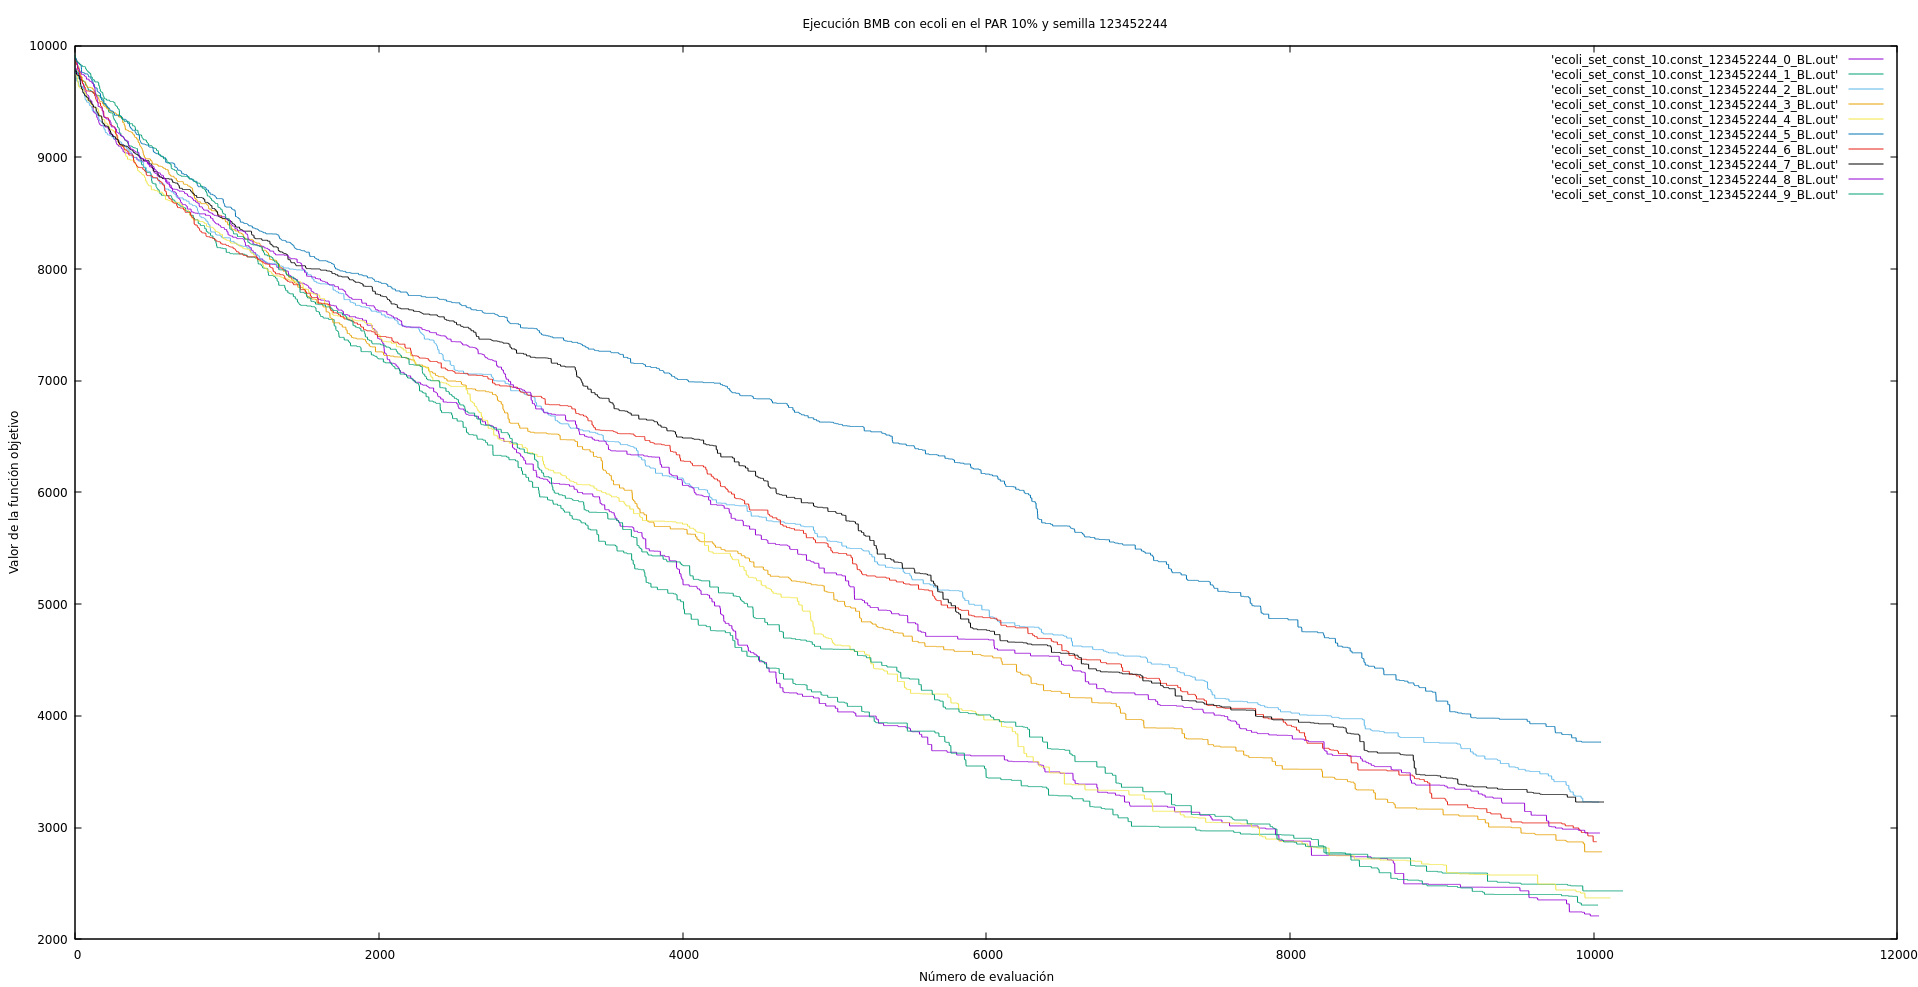
\includegraphics[scale = 0.40]{bmb-ecoli.png}
	
	\caption{BMB en ecoli.}
	\label{fig:bmb-cmp1}
\end{figure}

\begin{figure}[H]
	\centering
	\hspace*{-1.7cm}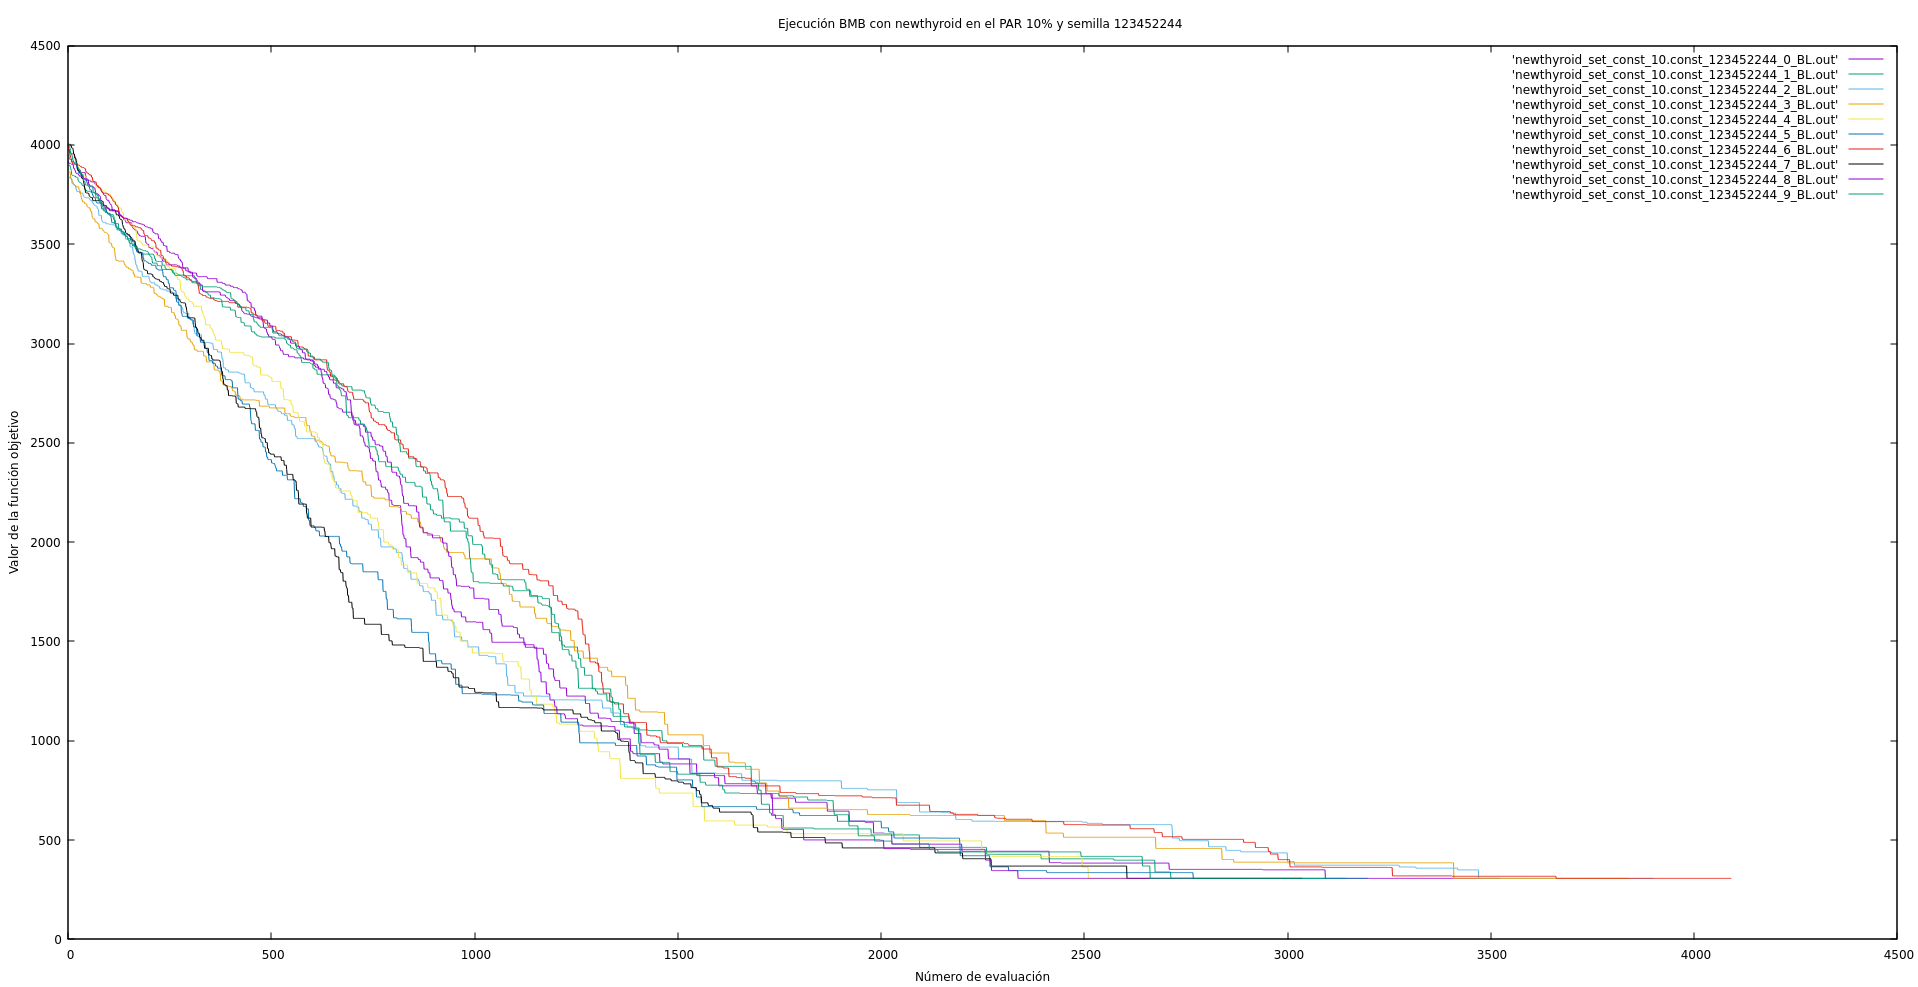
\includegraphics[scale = 0.40]{bmb-newthyroid.png}
	
	\caption{BMB en newthyroid.}
	\label{fig:bmb-cmp2}
\end{figure}


En estas imágenes vemos como en ecoli si utiliza las 10.000 evaluaciones de la BL mientras que en newthyroid (conjunto bastante más difícil que iris o rand) con unas 4.000 evaluaciones converge y encuentra una buena solución, lo que nos lleva a que tenga sentido ejecutar este algoritmo para este conjunto de datos. 

Si recordamos, en la práctica 1, ecoli necesitaba unas 35.000 evaluaciones para converger, luego usando este método con tan solo 10.000 evaluaciones no es capaz de converger y por lo tanto cualquier BL con más evaluaciones será mejor, es decir, en este conjunto de datos el intentar equilibrar exploración/explotación usando la búsqueda multiarranque básica hace que el nivel de explotación se vea tan afectado que no podamos obtener soluciones tan buenas como en otros algoritmos.

Recalcar que a pesar de esto, el algoritmo se comporta como se esperaba y como vemos en las tablas y en la imagen de newthyroid, hace obtener buenas soluciones siempre que los parámetros de ejecución sean los correctos para el conjunto de datos.

\subsubsection{ES-Proporcional.}

% Please add the following required packages to your document preamble:
% \usepackage{multirow}
\begin{table}[H]
\begin{tabular}{|c|c|c|c|c|c|c|c|c|}
\hline
\multicolumn{9}{|c|}{\textbf{Resultados obtenidos con el algoritmo ES-Pro en el PAR con un 10\% de restricciones}}                                                                                                \\ \hline
\multirow{2}{*}{} & \multicolumn{4}{c|}{\textbf{Iris}}                                                            & \multicolumn{4}{c|}{\textbf{Ecoli}}                                                           \\ \cline{2-9} 
                  & \textit{\textbf{Tasa\_C}} & \textit{\textbf{Tasa\_inf}} & \textit{\textbf{Agr,}} & \textbf{T} & \textit{\textbf{Tasa\_C}} & \textit{\textbf{Tasa\_inf}} & \textit{\textbf{Agr,}} & \textbf{T} \\ \hline
123452244         & 0,595316                  & 0                           & 0,595316               & 1,29613    & 1002,45                   & 38                          & 1156,39                & 14,5436    \\ \hline
9398429           & 0,595316                  & 0                           & 0,595316               & 1,52742    & 1013,11                   & 19                          & 1090,08                & 15,1577    \\ \hline
12321             & 0,595316                  & 0                           & 0,595316               & 1,55172    & 1048,96                   & 21                          & 1134,03                & 16,5802    \\ \hline
213566            & 0,595316                  & 0                           & 0,595316               & 1,47763    & 1048,2                    & 15                          & 1108,97                & 14,1945    \\ \hline
3939021           & 0,595316                  & 0                           & 0,595316               & 1,6313     & 1020,35                   & 27                          & 1129,73                & 14,606     \\ \hline
\textbf{Media}    & 0,595316                  & 0                           & 0,595316               & 1,49684    & 1026,614                  & 24                          & 1123,84                & 15,0164    \\ \hline
\end{tabular}
\end{table}


% Please add the following required packages to your document preamble:
% \usepackage{multirow}
\begin{table}[H]
\begin{tabular}{|c|c|c|c|c|c|c|c|c|}
\hline
\multicolumn{9}{|c|}{\textbf{Resultados obtenidos con el algoritmo ES-Pro en el PAR con un 10\% de restricciones}}                                                                                                \\ \hline
\multirow{2}{*}{} & \multicolumn{4}{c|}{\textbf{Rand}}                                                            & \multicolumn{4}{c|}{\textbf{Newthyroid}}                                                      \\ \cline{2-9} 
                  & \textit{\textbf{Tasa\_C}} & \textit{\textbf{Tasa\_inf}} & \textit{\textbf{Agr,}} & \textbf{T} & \textit{\textbf{Tasa\_C}} & \textit{\textbf{Tasa\_inf}} & \textit{\textbf{Agr,}} & \textbf{T} \\ \hline
123452244         & 0,746683                  & 0                           & 0,746683               & 1,3056     & 288,636                   & 6                           & 307,093                & 5,19199    \\ \hline
9398429           & 0,746683                  & 0                           & 0,746683               & 1,43435    & 288,636                   & 6                           & 307,093                & 6,2173     \\ \hline
12321             & 0,746683                  & 0                           & 0,746683               & 1,36369    & 288,636                   & 6                           & 307,093                & 5,60001    \\ \hline
213566            & 0,746683                  & 0                           & 0,746683               & 1,35742    & 288,636                   & 6                           & 307,093                & 5,71115    \\ \hline
3939021           & 0,746683                  & 0                           & 0,746683               & 1,80185    & 288,636                   & 6                           & 307,093                & 7,02851    \\ \hline
\textbf{Media}    & 0,746683                  & 0                           & 0,746683               & 1,4893275  & 288,636                   & 6                           & 307,093                & 5,949792   \\ \hline
\end{tabular}
\end{table}


% Please add the following required packages to your document preamble:
% \usepackage{multirow}
\begin{table}[H]
\begin{tabular}{|c|c|c|c|c|c|c|c|c|}
\hline
\multicolumn{9}{|c|}{\textbf{Resultados obtenidos con el algoritmo ES-Pro en el PAR con un 20\% de restricciones}}                                                                                                \\ \hline
\multirow{2}{*}{} & \multicolumn{4}{c|}{\textbf{Iris}}                                                            & \multicolumn{4}{c|}{\textbf{Ecoli}}                                                           \\ \cline{2-9} 
                  & \textit{\textbf{Tasa\_C}} & \textit{\textbf{Tasa\_inf}} & \textit{\textbf{Agr,}} & \textbf{T} & \textit{\textbf{Tasa\_C}} & \textit{\textbf{Tasa\_inf}} & \textit{\textbf{Agr,}} & \textbf{T} \\ \hline
123452244         & 0,595316                  & 0                           & 0,595316               & 2,03252    & 992,77                    & 71                          & 1136,59                & 15,9046    \\ \hline
9398429           & 0,595316                  & 0                           & 0,595316               & 2,00236    & 1010,66                   & 78                          & 1168,65                & 15,5202    \\ \hline
12321             & 0,595316                  & 0                           & 0,595316               & 1,64673    & 1030,19                   & 81                          & 1194,27                & 17,2348    \\ \hline
213566            & 0,595316                  & 0                           & 0,595316               & 1,81872    & 1043,61                   & 49                          & 1142,86                & 14,4862    \\ \hline
3939021           & 0,595316                  & 0                           & 0,595316               & 1,67148    & 1043,57                   & 79                          & 1203,59                & 16,3528    \\ \hline
\textbf{Media}    & 0,595316                  & 0                           & 0,595316               & 1,834362   & 1024,16                   & 71,6                        & 1169,192               & 15,89972   \\ \hline
\end{tabular}
\end{table}


% Please add the following required packages to your document preamble:
% \usepackage{multirow}
\begin{table}[H]
\begin{tabular}{|c|c|c|c|c|c|c|c|c|}
\hline
\multicolumn{9}{|c|}{\textbf{Resultados obtenidos con el algoritmo ES-Pro en el PAR con un 20\% de restricciones}}                                                                                                \\ \hline
\multirow{2}{*}{} & \multicolumn{4}{c|}{\textbf{Rand}}                                                            & \multicolumn{4}{c|}{\textbf{Newthyroid}}                                                      \\ \cline{2-9} 
                  & \textit{\textbf{Tasa\_C}} & \textit{\textbf{Tasa\_inf}} & \textit{\textbf{Agr,}} & \textbf{T} & \textit{\textbf{Tasa\_C}} & \textit{\textbf{Tasa\_inf}} & \textit{\textbf{Agr,}} & \textbf{T} \\ \hline
123452244         & 0,746683                  & 0                           & 0,746683               & 1,81453    & 313,299                   & 0                           & 313,299                & 6,57469    \\ \hline
9398429           & 0,746683                  & 0                           & 0,746683               & 1,5968     & 313,299                   & 0                           & 313,299                & 7,30788    \\ \hline
12321             & 0,746683                  & 0                           & 0,746683               & 1,66481    & 313,299                   & 0                           & 313,299                & 6,51556    \\ \hline
213566            & 0,746683                  & 0                           & 0,746683               & 1,64302    & 313,299                   & 0                           & 313,299                & 6,84998    \\ \hline
3939021           & 0,746683                  & 0                           & 0,746683               & 1,85641    & 313,299                   & 0                           & 313,299                & 5,25557    \\ \hline
\textbf{Media}    & 0,746683                  & 0                           & 0,746683               & 1,715114   & 313,299                   & 0                           & 313,299                & 6,500736   \\ \hline
\end{tabular}
\end{table}


Con  algoritmo de enfriamiento simulado se intenta buscar una gran exploración al inicio del algoritmo, y según este avanza explotar la solución encontrada, de forma que si en el proceso de exploración encuentra una zona del espacio de búsqueda prometedora, aunque la temperatura sea alta la explorará ya que obtendrá mejor solución, aunque podrá salir de esa zona por la temperatura. Por el contrario, si el algoritmo ya está lo suficientemente avanzado, la temperatura será más baja e intentará explotar esa zona para que esa sea su mejor solución.

Como comente en la implementación del algoritmo, modifique el esquema de enfriamiento pasando a usar el esquema proporcional en lugar del esquema de Cauchy modificado debido a que este último realizaba un enfriamiento demasiado brusco. Ese enfriamiento brusco no permitía tener el equilibrio exploración/exploración que se buscaba y por eso decidí realizar este cambio. Lo justificare en detalle en la sección de otros experimentos donde realizaré un análisis más exhaustivo de la importancia de escoger un buen criterio de enfriamiento.

Viendo los resultados de las tablas vemos como parece que las soluciones son bastante buenas en las distintas semillas y casos, sin embargo las tablas no nos permiten ver si el algoritmo se comporta como esperábamos, por eso me basaré en imágenes para explicar el comportamiento:

\begin{figure}[H]
	\centering
	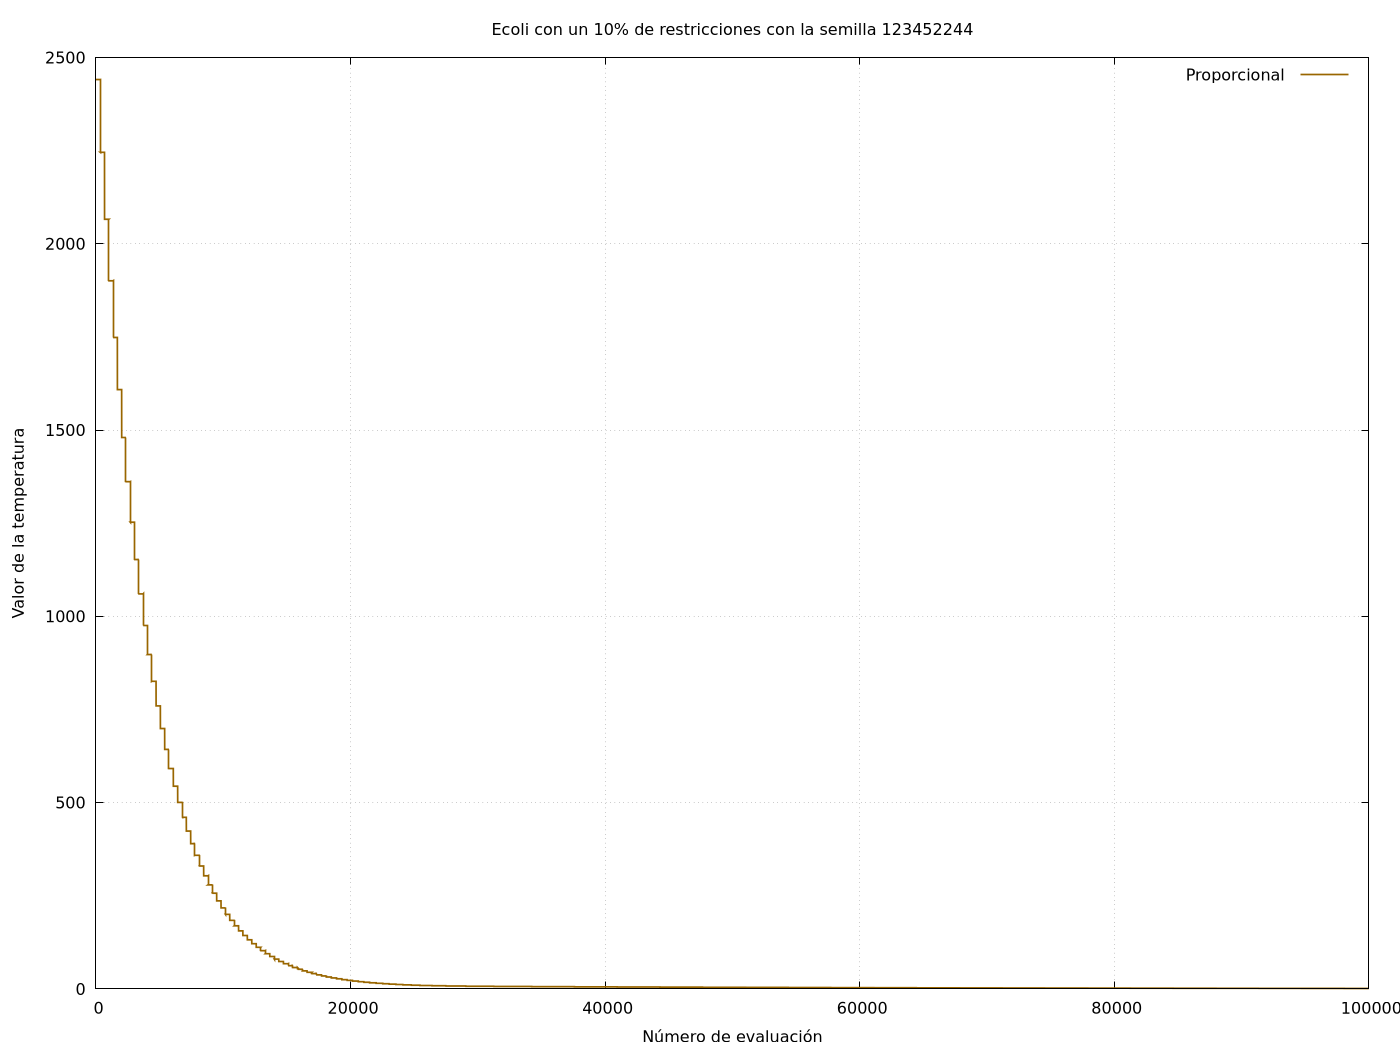
\includegraphics[scale = 0.35]{es-temp-ecoli-10.png}
	
	\caption{Temperatura en ES-PRO en ecoli.}
	\label{fig:es-cmp2}
\end{figure}

\begin{figure}[H]
	\centering
	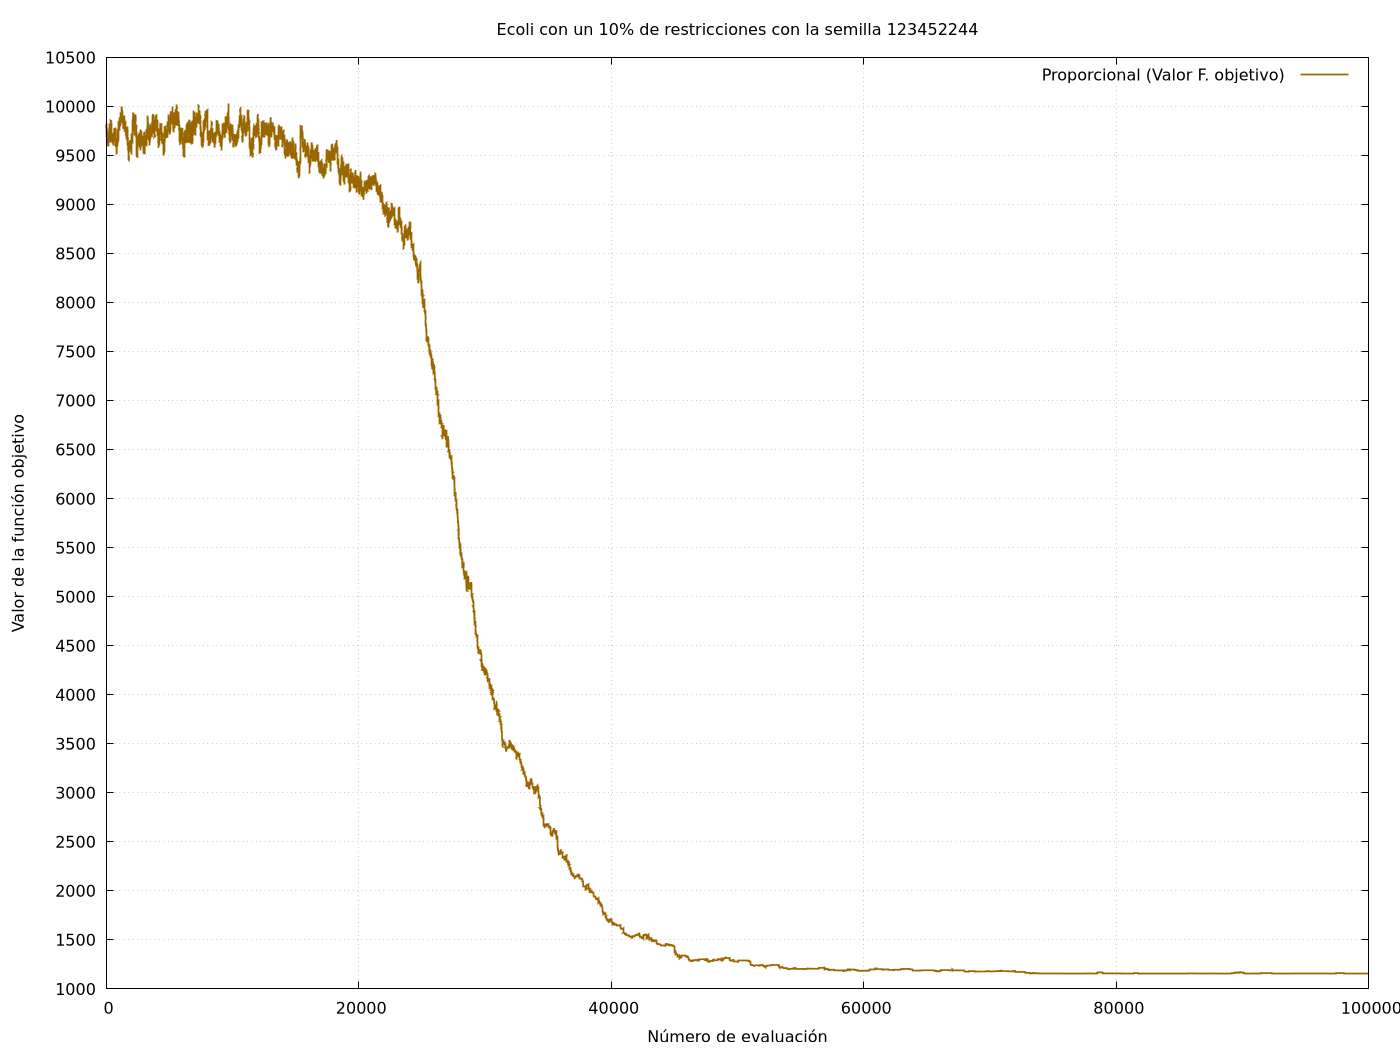
\includegraphics[scale = 0.35]{es-ecoli-10.png}
	
	\caption{Función objetivo en ES-PRO en ecoli.}
	\label{fig:es-cmp1}
\end{figure}


Para comentar el algoritmo he utilizado la ejecución en ecoli con un 10\% de restricciones, aunque en todos los conjuntos de datos se comporta correctamente y se puede comprobar en los png que se pueden generar en la carpeta gráficas tras ejecutar los algoritmos (aun así los adjunto en la entrega en la carpeta de gráficas/salidas\_png). He escogido este conjunto ya que se marca claramente el avance.

En la primera imagen vemos como avanza la temperatura en la ejecución, mientras que en la segunda el valor de la función objetivo de la solución actual. Estas imágenes tenemos que interpretarlas juntas. Vemos como al inicio, en las primeras 20.000 evaluaciones donde la temperatura es alta, el valor de la función objetivo va tomando distintos valores y hay pequeñas zonas donde se reduce y otras donde aumenta, dando lugar a esa exploración del espacio de búsqueda, mientras que en las siguientes evaluaciones, cuando la temperatura cae, la explotación se intensifica y converge a una solución bastante buena.

El que la temperatura sea baja no impide que acepte peores soluciones, en ocasiones, como vemos alrededor de la evaluación 40.000 se aceptan soluciones peores, o incluso cerca de la evaluación 90.000 se siguen aceptando soluciones un poco peores, pero como vemos por el criterio de Metrópolis, la diferencia de estas soluciones con respecto a la actual es cada vez más pequeña, por lo que el comportamiento es correcto y como vemos logramos un resultado bastante bueno.

\subsubsection{ILS.}


% Please add the following required packages to your document preamble:
% \usepackage{multirow}
\begin{table}[H]
\begin{tabular}{|c|c|c|c|c|c|c|c|c|}
\hline
\multicolumn{9}{|c|}{\textbf{Resultados obtenidos con el algoritmo ILS en el PAR con un 10\% de restricciones}}                                                                                                   \\ \hline
\multirow{2}{*}{} & \multicolumn{4}{c|}{\textbf{Iris}}                                                            & \multicolumn{4}{c|}{\textbf{Ecoli}}                                                           \\ \cline{2-9} 
                  & \textit{\textbf{Tasa\_C}} & \textit{\textbf{Tasa\_inf}} & \textit{\textbf{Agr,}} & \textbf{T} & \textit{\textbf{Tasa\_C}} & \textit{\textbf{Tasa\_inf}} & \textit{\textbf{Agr,}} & \textbf{T} \\ \hline
123452244         & 0,595316                  & 0                           & 0,595316               & 0,273917   & 1009,08                   & 21                          & 1094,15                & 4,04542    \\ \hline
9398429           & 0,595316                  & 0                           & 0,595316               & 0,261119   & 1008,44                   & 26                          & 1113,77                & 4,43429    \\ \hline
12321             & 0,595316                  & 0                           & 0,595316               & 0,293068   & 973,033                   & 40                          & 1135,08                & 5,1826     \\ \hline
213566            & 0,595316                  & 0                           & 0,595316               & 0,278702   & 1057,8                    & 31                          & 1183,39                & 4,38417    \\ \hline
3939021           & 0,595316                  & 0                           & 0,595316               & 0,27003    & 997,708                   & 26                          & 1103,04                & 4,86433    \\ \hline
\textbf{Media}    & 0,595316                  & 0                           & 0,595316               & 0,2753672  & 1009,2122                 & 28,8                        & 1125,886               & 4,582162   \\ \hline
\end{tabular}
\end{table}

% Please add the following required packages to your document preamble:
% \usepackage{multirow}
\begin{table}[H]
\begin{tabular}{|c|c|c|c|c|c|c|c|c|}
\hline
\multicolumn{9}{|c|}{\textbf{Resultados obtenidos con el algoritmo ILS en el PAR con un 10\% de restricciones}}                                                                                                   \\ \hline
\multirow{2}{*}{} & \multicolumn{4}{c|}{\textbf{Rand}}                                                            & \multicolumn{4}{c|}{\textbf{Newthyroid}}                                                      \\ \cline{2-9} 
                  & \textit{\textbf{Tasa\_C}} & \textit{\textbf{Tasa\_inf}} & \textit{\textbf{Agr,}} & \textbf{T} & \textit{\textbf{Tasa\_C}} & \textit{\textbf{Tasa\_inf}} & \textit{\textbf{Agr,}} & \textbf{T} \\ \hline
123452244         & 0,746683                  & 0                           & 0,746683               & 0,293904   & 288,636                   & 6                           & 307,093                & 0,601991   \\ \hline
9398429           & 0,746683                  & 0                           & 0,746683               & 0,230752   & 288,636                   & 6                           & 307,093                & 0,851253   \\ \hline
12321             & 0,746683                  & 0                           & 0,746683               & 0,301232   & 288,636                   & 6                           & 307,093                & 1,15655    \\ \hline
213566            & 0,746683                  & 0                           & 0,746683               & 0,258103   & 288,636                   & 6                           & 307,093                & 1,08858    \\ \hline
3939021           & 0,746683                  & 0                           & 0,746683               & 0,31106    & 288,636                   & 6                           & 307,093                & 0,97528    \\ \hline
\textbf{Media}    & 0,746683                  & 0                           & 0,746683               & 0,27528675 & 288,636                   & 6                           & 307,093                & 0,9347308  \\ \hline
\end{tabular}
\end{table}


% Please add the following required packages to your document preamble:
% \usepackage{multirow}
\begin{table}[H]
\begin{tabular}{|c|c|c|c|c|c|c|c|c|}
\hline
\multicolumn{9}{|c|}{\textbf{Resultados obtenidos con el algoritmo ILS en el PAR con un 20\% de restricciones}}                                                                                                   \\ \hline
\multirow{2}{*}{} & \multicolumn{4}{c|}{\textbf{Iris}}                                                            & \multicolumn{4}{c|}{\textbf{Ecoli}}                                                           \\ \cline{2-9} 
                  & \textit{\textbf{Tasa\_C}} & \textit{\textbf{Tasa\_inf}} & \textit{\textbf{Agr,}} & \textbf{T} & \textit{\textbf{Tasa\_C}} & \textit{\textbf{Tasa\_inf}} & \textit{\textbf{Agr,}} & \textbf{T} \\ \hline
123452244         & 0,595316                  & 0                           & 0,595316               & 0,307581   & 972,608                   & 73                          & 1120,48                & 5,27057    \\ \hline
9398429           & 0,595316                  & 0                           & 0,595316               & 0,335643   & 1025,54                   & 88                          & 1203,79                & 6,24117    \\ \hline
12321             & 0,595316                  & 0                           & 0,595316               & 0,368848   & 1004,19                   & 65                          & 1135,86                & 6,43785    \\ \hline
213566            & 0,595316                  & 0                           & 0,595316               & 0,358544   & 961,608                   & 56                          & 1075,04                & 5,43663    \\ \hline
3939021           & 0,595316                  & 0                           & 0,595316               & 0,321154   & 1038,98                   & 61                          & 1162,54                & 6,47105    \\ \hline
\textbf{Media}    & 0,595316                  & 0                           & 0,595316               & 0,338354   & 1000,5852                 & 68,6                        & 1139,542               & 5,971454   \\ \hline
\end{tabular}
\end{table}


% Please add the following required packages to your document preamble:
% \usepackage{multirow}
\begin{table}[H]
\begin{tabular}{|c|c|c|c|c|c|c|c|c|}
\hline
\multicolumn{9}{|c|}{\textbf{Resultados obtenidos con el algoritmo ILS en el PAR con un 20\% de restricciones}}                                                                                                   \\ \hline
\multirow{2}{*}{} & \multicolumn{4}{c|}{\textbf{Rand}}                                                            & \multicolumn{4}{c|}{\textbf{Newthyroid}}                                                      \\ \cline{2-9} 
                  & \textit{\textbf{Tasa\_C}} & \textit{\textbf{Tasa\_inf}} & \textit{\textbf{Agr,}} & \textbf{T} & \textit{\textbf{Tasa\_C}} & \textit{\textbf{Tasa\_inf}} & \textit{\textbf{Agr,}} & \textbf{T} \\ \hline
123452244         & 0,746683                  & 0                           & 0,746683               & 0,354395   & 313,299                   & 0                           & 313,299                & 1,02242    \\ \hline
9398429           & 0,746683                  & 0                           & 0,746683               & 0,32391    & 313,299                   & 0                           & 313,299                & 0,921081   \\ \hline
12321             & 0,746683                  & 0                           & 0,746683               & 0,362464   & 313,299                   & 0                           & 313,299                & 1,35868    \\ \hline
213566            & 0,746683                  & 0                           & 0,746683               & 0,327969   & 313,299                   & 0                           & 313,299                & 0,914066   \\ \hline
3939021           & 0,746683                  & 0                           & 0,746683               & 0,318336   & 313,299                   & 0                           & 313,299                & 1,12753    \\ \hline
\textbf{Media}    & 0,746683                  & 0                           & 0,746683               & 0,33316975 & 313,299                   & 0                           & 313,299                & 1,0687554  \\ \hline
\end{tabular}
\end{table}

La ILS, ejecutada con parámetros de 10 iteraciones y cada iteración una BL de 10.000 evaluaciones vemos que obtenemos soluciones bastante buenas, pero de nuevo, en las tablas no somos capaces de evaluar el comportamiento del algoritmo. Por este motivo, una traza de la ejecución sobre ecoli es esta:

\begin{figure}[H]
	\centering
	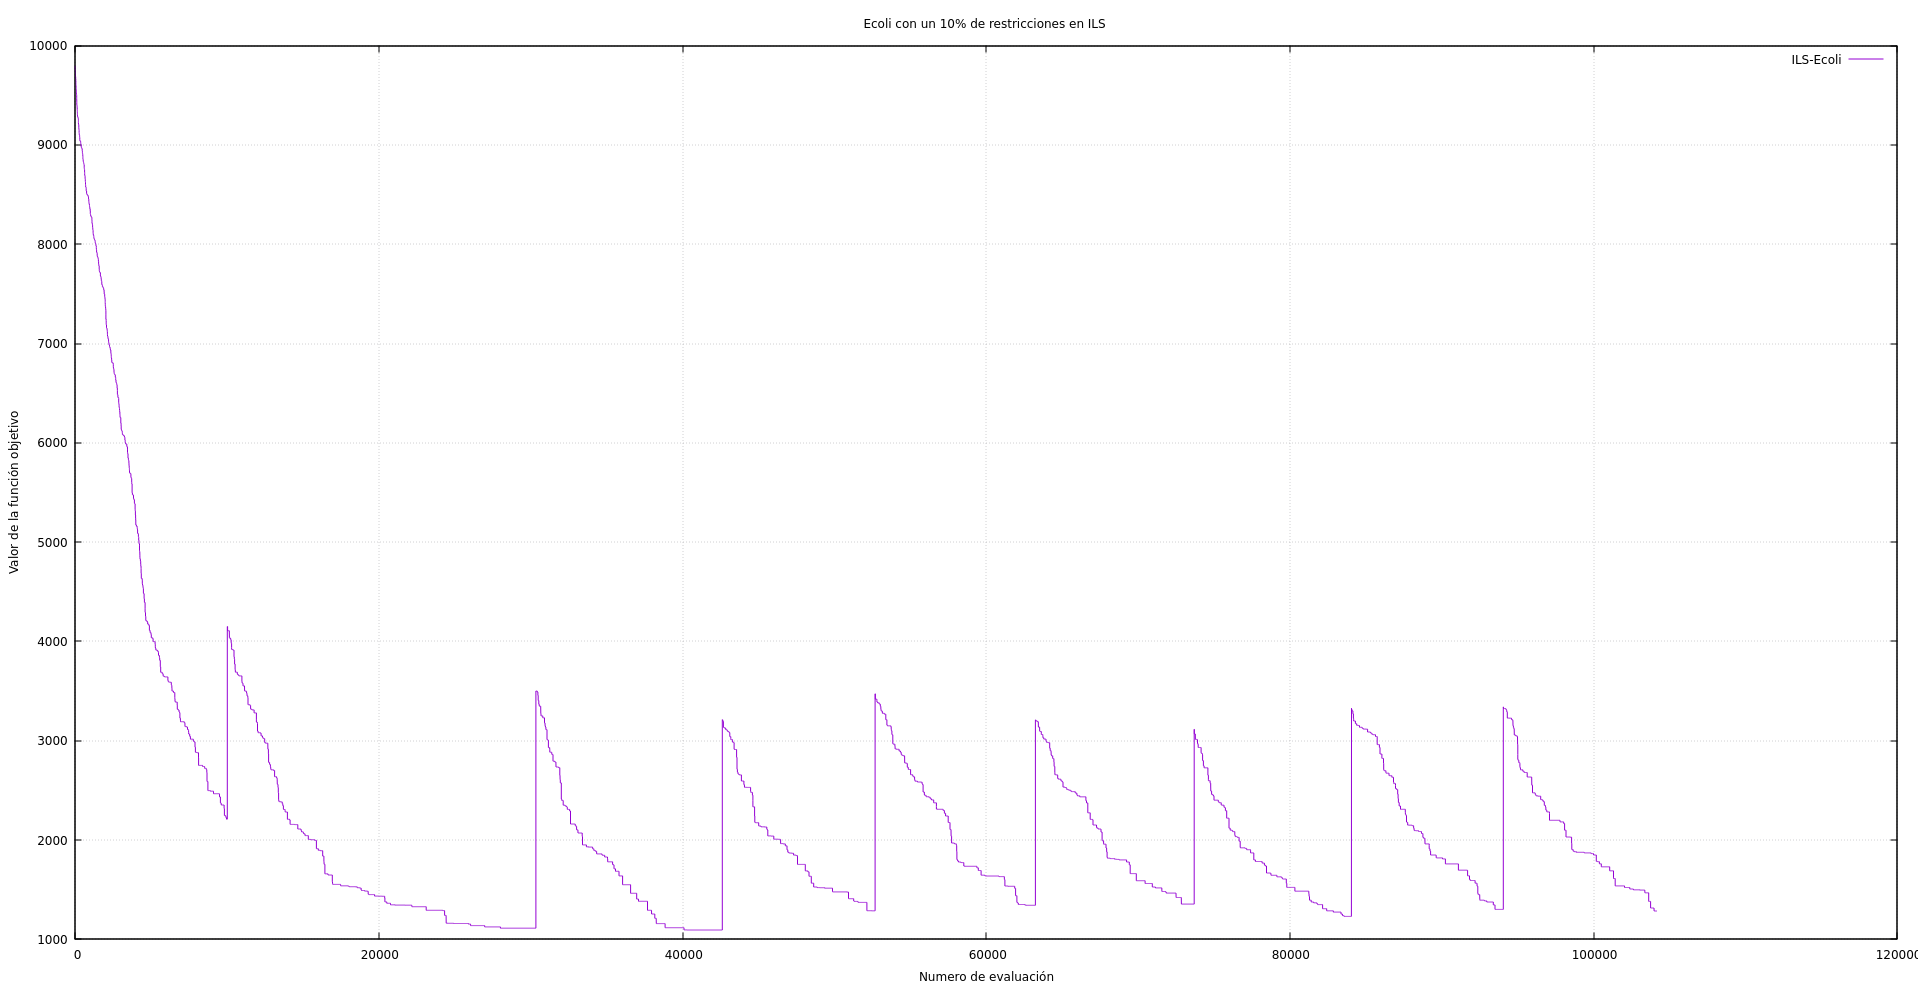
\includegraphics[scale = 0.35]{ecoli-ils.png}
	
	\caption{Función objetivo en ILS en ecoli.}
	\label{fig:ils-cmp1}
\end{figure}

De nuevo he usado ecoli ya que los otros conjuntos de datos el algoritmo se comporta bien pero al necesitar menos evaluaciones para converger se hace menos visual el comportamiento del algoritmo.

Vemos como en las dos primeras ejecuciones utiliza un poco más de las 10.000 evaluaciones, ya que en la búsqueda local permitíamos esto para no tener que detener la ejecución en mitad de la exploración de un vecindario, pero al partir de una solución parecida y no una totalmente nueva como en el caso de BMB, evitamos precisamente el problema de la BMB de no tener suficientes iteraciones para converger y antes de realizar la segunda mutación ya encuentra un mínimo local.

En cada ejecución de la búsqueda local vemos como la mutación funciona y modifica la solución lo suficiente como para que el siguiente mínimo sea distinto al anterior, por lo que el algoritmo cumple con su objetivo y es capaz de moverse por las zonas del espacio cuando cae en un mínimo.

Esto funciona ya que sabemos que la búsqueda local nos va a encontrar el mejor de su entorno y vamos a llegar a mínimos locales. 

Hay que tener muy en cuenta los parámetros con los que ejecutamos el algoritmo ILS, en especial el porcentaje de solución a mutar, ya que tenemos tres escenarios:

\begin{enumerate}
	\item \textbf{Porcentaje a mutar demasiado alto con respecto al número de evaluaciones de cada BL}: Cada vez que ejecutemos la mutación se la solución será muy distinta a la que teníamos, por lo tanto, cada BL necesitará más evaluaciones con el fin de llegar a un mínimo, y si no cuenta con ese mínimo de evaluaciones nunca convergeremos, dando malas soluciones.
	\item \textbf{Porcentaje a mutar acorde a las evaluaciones de cada BL}: Este es el escenario que buscamos, los cambios en una solución son tan bruscos como para movernos a otra zona del espacio de búsqueda, sin embargo siguen permitiendo a la BL llegar a un mínimo local.
	\item \textbf{Porcentaje de cambios muy bajo}: El cambio apenas es brusco, por lo que la solución se mantendrá en la misma zona del espacio, haciendo que este algoritmo no explore, y por lo tanto sea equivalente a única BL.
\end{enumerate}


Es importante tener en cuenta que la mutación, al ser un porcentaje de la solución, se adapta bien a los conjuntos de datos, esto lo podemos ver en como se comporta en iris:

\begin{figure}[H]
	\centering
	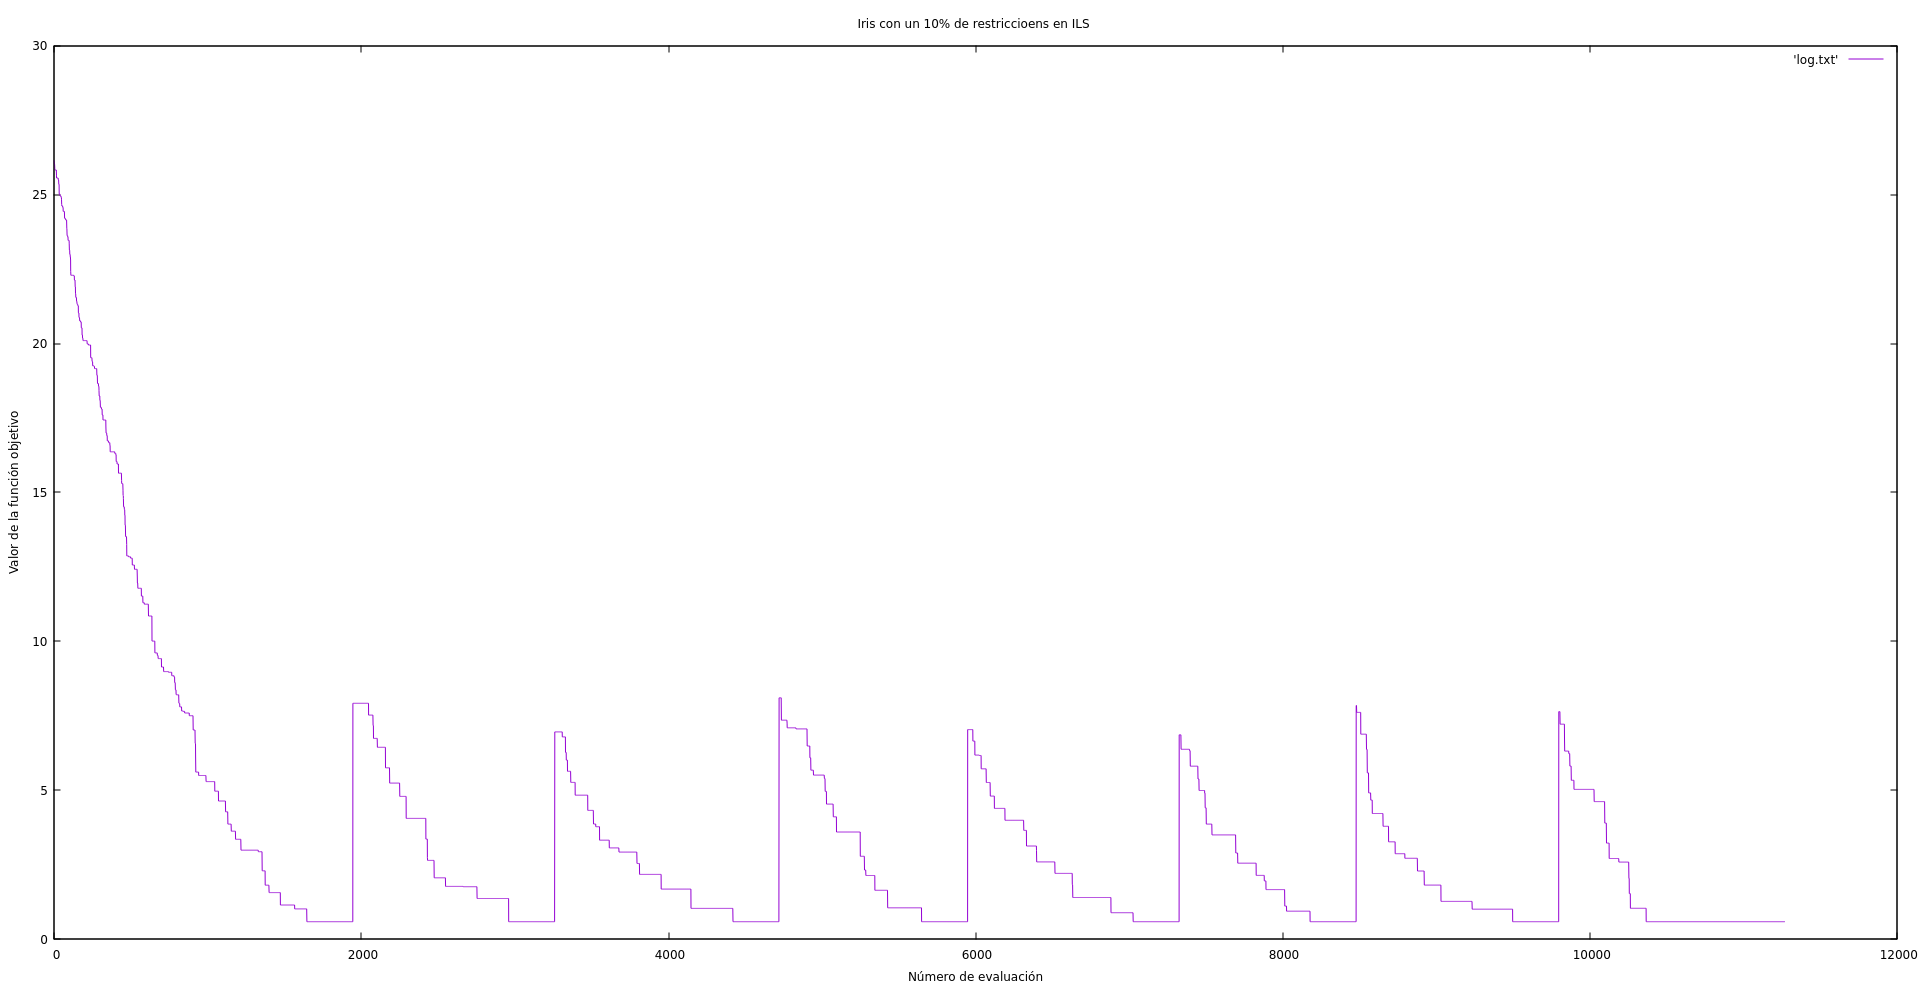
\includegraphics[scale = 0.35]{iris-ils.png}
	
	\caption{Función objetivo en ILS en iris.}
	\label{fig:ils-cmp2}
\end{figure}

Vemos como se sigue comportando de forma correcta, ya que llega a un mínimo, por lo que al aplicar la mutación no supone irnos a una solución muy mala.

\subsubsection{ILS-ES.}

% Please add the following required packages to your document preamble:
% \usepackage{multirow}
\begin{table}[H]
\begin{tabular}{|c|c|c|c|c|c|c|c|c|}
\hline
\multicolumn{9}{|c|}{\textbf{Resultados obtenidos con el algoritmo ILS-ES en el PAR con un 10\% de restricciones}}                                                                                                \\ \hline
\multirow{2}{*}{} & \multicolumn{4}{c|}{\textbf{Iris}}                                                            & \multicolumn{4}{c|}{\textbf{Ecoli}}                                                           \\ \cline{2-9} 
                  & \textit{\textbf{Tasa\_C}} & \textit{\textbf{Tasa\_inf}} & \textit{\textbf{Agr,}} & \textbf{T} & \textit{\textbf{Tasa\_C}} & \textit{\textbf{Tasa\_inf}} & \textit{\textbf{Agr,}} & \textbf{T} \\ \hline
123452244         & 0,595316                  & 0                           & 0,595316               & 4,07449    & 2339,45                   & 1737                        & 9376,34                & 7,22955    \\ \hline
9398429           & 0,595316                  & 0                           & 0,595316               & 4,3089     & 2358,5                    & 1724                        & 9342,72                & 7,56503    \\ \hline
12321             & 0,595316                  & 0                           & 0,595316               & 5,76516    & 2320,9                    & 1718                        & 9280,82                & 8,16927    \\ \hline
213566            & 0,595316                  & 0                           & 0,595316               & 5,54703    & 2316,77                   & 1721                        & 9288,84                & 7,62729    \\ \hline
3939021           & 0,595316                  & 0                           & 0,595316               & 5,45429    & 2311,14                   & 1735                        & 9339,93                & 7,58435    \\ \hline
\textbf{Media}    & 0,595316                  & 0                           & 0,595316               & 5,029974   & 2329,352                  & 1727                        & 9325,73                & 7,635098   \\ \hline
\end{tabular}
\end{table}


% Please add the following required packages to your document preamble:
% \usepackage{multirow}
\begin{table}[H]
\begin{tabular}{|c|c|c|c|c|c|c|c|c|}
\hline
\multicolumn{9}{|c|}{\textbf{Resultados obtenidos con el algoritmo ILS-ES en el PAR con un 10\% de restricciones}}                                                                                                \\ \hline
\multirow{2}{*}{} & \multicolumn{4}{c|}{\textbf{Rand}}                                                            & \multicolumn{4}{c|}{\textbf{Newthyroid}}                                                      \\ \cline{2-9} 
                  & \textit{\textbf{Tasa\_C}} & \textit{\textbf{Tasa\_inf}} & \textit{\textbf{Agr,}} & \textbf{T} & \textit{\textbf{Tasa\_C}} & \textit{\textbf{Tasa\_inf}} & \textit{\textbf{Agr,}} & \textbf{T} \\ \hline
123452244         & 0,746683                  & 0                           & 0,746683               & 4,17904    & 297,55                    & 1023                        & 3444,45                & 5,35405    \\ \hline
9398429           & 0,746683                  & 0                           & 0,746683               & 4,11659    & 311,963                   & 991                         & 3360,43                & 6,79565    \\ \hline
12321             & 0,746683                  & 0                           & 0,746683               & 5,64873    & 305,157                   & 992                         & 3356,7                 & 7,24503    \\ \hline
213566            & 0,746683                  & 0                           & 0,746683               & 5,29604    & 305,012                   & 994                         & 3362,71                & 6,52566    \\ \hline
3939021           & 0,746683                  & 0                           & 0,746683               & 5,72909    & 319,445                   & 928                         & 3174,11                & 7,55266    \\ \hline
\textbf{Media}    & 0,746683                  & 0                           & 0,746683               & 5,1976125  & 307,8254                  & 985,6                       & 3339,68                & 6,69461    \\ \hline
\end{tabular}
\end{table}


% Please add the following required packages to your document preamble:
% \usepackage{multirow}
\begin{table}[H]
\begin{tabular}{|c|c|c|c|c|c|c|c|c|}
\hline
\multicolumn{9}{|c|}{\textbf{Resultados obtenidos con el algoritmo ILS-ES en el PAR con un 20\% de restricciones}}                                                                                                \\ \hline
\multirow{2}{*}{} & \multicolumn{4}{c|}{\textbf{Iris}}                                                            & \multicolumn{4}{c|}{\textbf{Ecoli}}                                                           \\ \cline{2-9} 
                  & \textit{\textbf{Tasa\_C}} & \textit{\textbf{Tasa\_inf}} & \textit{\textbf{Agr,}} & \textbf{T} & \textit{\textbf{Tasa\_C}} & \textit{\textbf{Tasa\_inf}} & \textit{\textbf{Agr,}} & \textbf{T} \\ \hline
123452244         & 0,595316                  & 0                           & 0,595316               & 4,63981    & 2326,97                   & 3475                        & 9365,88                & 8,50748    \\ \hline
9398429           & 0,595316                  & 0                           & 0,595316               & 5,41024    & 2319,32                   & 3477                        & 9362,28                & 9,23918    \\ \hline
12321             & 0,595316                  & 0                           & 0,595316               & 6,13119    & 2319,01                   & 3491                        & 9390,33                & 9,03569    \\ \hline
213566            & 0,595316                  & 0                           & 0,595316               & 5,90785    & 2294,73                   & 3491                        & 9366,05                & 8,76367    \\ \hline
3939021           & 0,595316                  & 0                           & 0,595316               & 6,21889    & 2340,55                   & 3468                        & 9365,28                & 8,66403    \\ \hline
\textbf{Media}    & 0,595316                  & 0                           & 0,595316               & 5,661596   & 2320,116                  & 3480,4                      & 9369,964               & 8,84201    \\ \hline
\end{tabular}
\end{table}


% Please add the following required packages to your document preamble:
% \usepackage{multirow}
\begin{table}[H]
\begin{tabular}{|c|c|c|c|c|c|c|c|c|}
\hline
\multicolumn{9}{|c|}{\textbf{Resultados obtenidos con el algoritmo ILS-ES en el PAR con un 20\% de restricciones}}                                                                                                \\ \hline
\multirow{2}{*}{} & \multicolumn{4}{c|}{\textbf{Rand}}                                                            & \multicolumn{4}{c|}{\textbf{Newthyroid}}                                                      \\ \cline{2-9} 
                  & \textit{\textbf{Tasa\_C}} & \textit{\textbf{Tasa\_inf}} & \textit{\textbf{Agr,}} & \textbf{T} & \textit{\textbf{Tasa\_C}} & \textit{\textbf{Tasa\_inf}} & \textit{\textbf{Agr,}} & \textbf{T} \\ \hline
123452244         & 0,746683                  & 0                           & 0,746683               & 4,72714    & 314,814                   & 2119                        & 3573,29                & 6,05776    \\ \hline
9398429           & 0,746683                  & 0                           & 0,746683               & 5,21703    & 318,796                   & 1922                        & 3274,34                & 7,16428    \\ \hline
12321             & 0,746683                  & 0                           & 0,746683               & 6,32949    & 319,039                   & 2025                        & 3432,97                & 8,58817    \\ \hline
213566            & 0,746683                  & 0                           & 0,746683               & 5,00052    & 315,753                   & 2041                        & 3454,28                & 7,2069     \\ \hline
3939021           & 0,746683                  & 0                           & 0,746683               & 6,49538    & 300,517                   & 2084                        & 3505,17                & 8,06598    \\ \hline
\textbf{Media}    & 0,746683                  & 0                           & 0,746683               & 5,760605   & 313,7838                  & 2038,2                      & 3448,01                & 7,416618   \\ \hline
\end{tabular}
\end{table}

Este algoritmo se basa de una hibridación del algoritmo ILS pero usando enfriamiento simulado en lugar de búsqueda local como algoritmo por trayectorias en cada iteración de la ILS. 

Aunque se ejecuta con los mismos parámetros que ILS (10 iteraciones de la ILS y 10.000 evaluaciones cada ejecución del ES), vemos como los resultados en este caso son igual de buenos en iris y rand, pero no en ecoli y newthyroid. Esto se debe al comportamiento y dificultad de cada conjunto de datos, por lo que compararemos a fondo el comportamiento comparando la ejecución en iris con la ejecución en ecoli:


\begin{figure}[H]
	\centering
	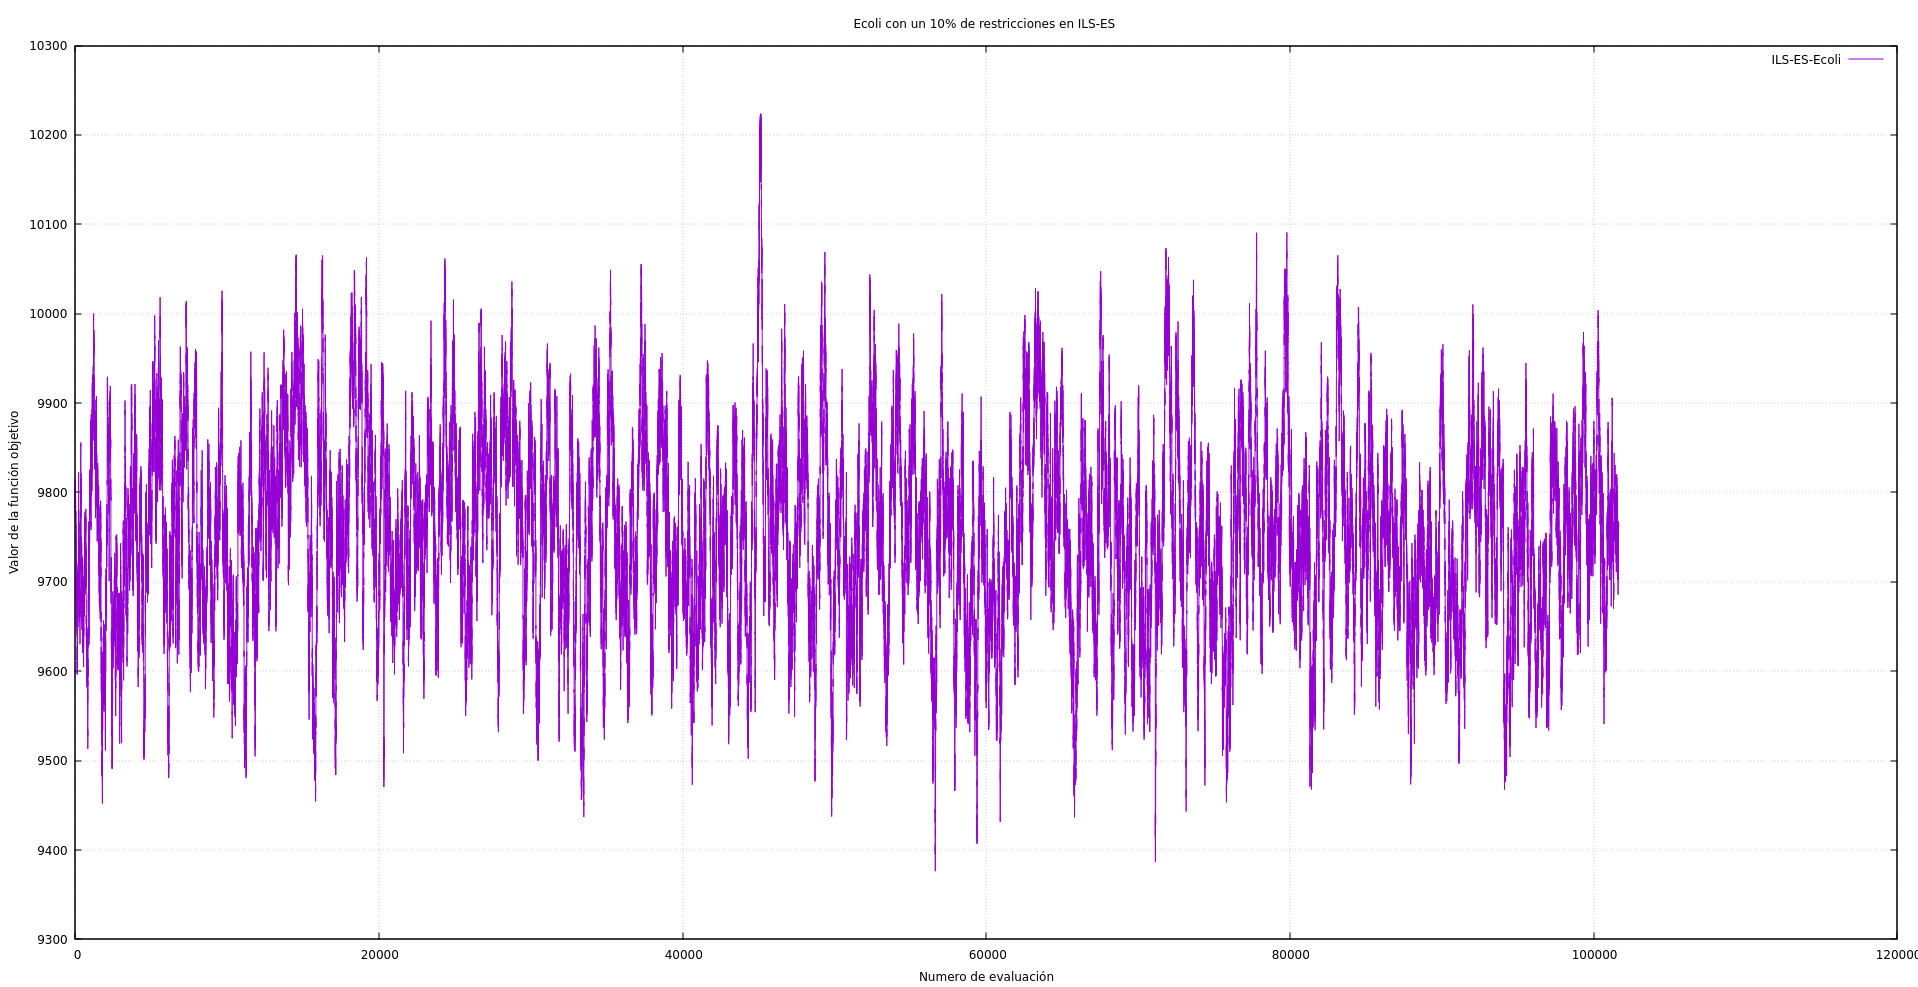
\includegraphics[scale = 0.35]{ecoli-ils-es.png}
	
	\caption{ILS-ES sobre ecoli con 10\% de restricciones.}
	\label{fig:es-cmp2}
\end{figure}

\begin{figure}[H]
	\centering
	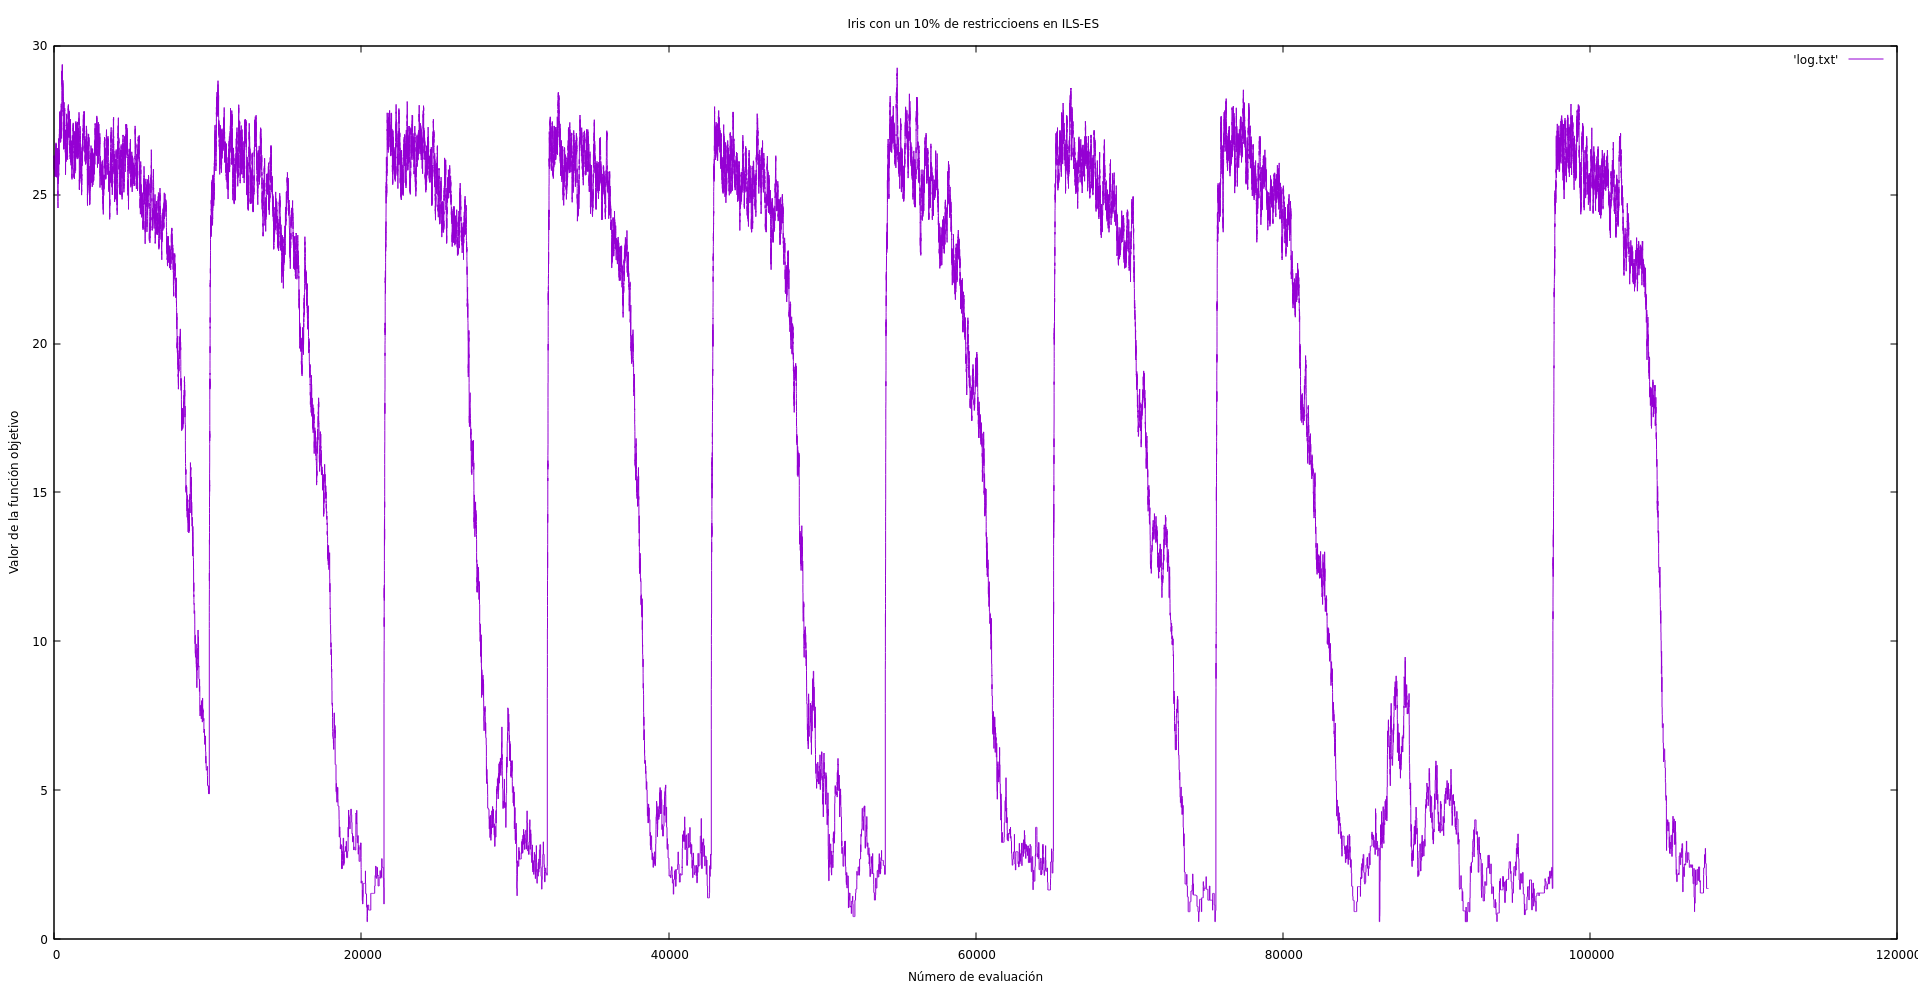
\includegraphics[scale = 0.35]{iris-ils-es.png}
	
	\caption{ILS-ES sobre ecoli con 10\% de restricciones.}
	\label{fig:es-cmp1}
\end{figure}

Vemos que en ambos casos hace más de 10.000 iteraciones en algunas ejecuciones, lo que hace que no sean exactamente el mismo número de evaluaciones, sin embargo si modifico esto no se realizarían en todos los casos las 10 mutaciones.

Como comente en enfriamiento simulado y entraré más a fondo más adelante, el criterio de enfriamiento es muy importante. En este ejemplo lo podemos ver, en un conjunto pequeño y sencillo como iris, las 10.000 evaluaciones son suficientes para lograr enfriar lo suficientemente rápido usando un esquema proporcional y ser capaces de dar una buena solución, aunque si es cierto que se introduce un nuevo problema, y es que estamos en el caso 3 que comenté en  el apartado de ILS. 

La búsqueda local es capaz de hacer converger rápidamente la solución de iris y entrar en un mínimo, por lo que al aplicar la mutación del 10\% la solución no empeora mucho. Por el contrario, en este caso, aunque el enfriamiento simulado llega a explotar, no hace la suficiente explotación como para converger a un mínimo, solo se acerca a este, por lo que la mutación en conjunto al error que contiene de por si la solución tiene como efecto que la solución con la que se trabaja sea prácticamente como una nueva solución, por lo que el comportamiento es el del algoritmo de BMB. 


Por el contrario, en ecoli, debido a la complejidad y tamaño del conjunto de datos, con 10.000 evaluaciones de enfriamiento simulado la temperatura sigue siendo tan alta que el algoritmo simplemente se reduce a explorar soluciones distintas, y no explotarlas, por lo que nos da soluciones muy malas y prácticamente aleatorias.

El caso de ecoli lo podríamos solucionar buscando un esquema de enfriamiento que enfríe más rápido, para que así en las 10.000 evaluaciones sea capaz de explotar y no simplemente explorar.


\subsection{Análisis de resultados.	}

\subsubsection{10\% de restricciones.}

% Please add the following required packages to your document preamble:
% \usepackage{multirow}
\begin{table}[H]
\begin{tabular}{|c|c|c|c|c|c|c|c|c|}
\hline
\multicolumn{9}{|c|}{\textbf{Resultados globales en el PAR con un 10\% de restricciones}}                                                                                                                      \\ \hline
\multicolumn{1}{|l|}{\multirow{2}{*}{}} & \multicolumn{4}{c|}{\textbf{Iris}}                                                            & \multicolumn{4}{c|}{\textbf{Ecoli}}                                                           \\ \cline{2-9} 
\multicolumn{1}{|l|}{}                  & \textit{\textbf{Tasa\_C}} & \textit{\textbf{Tasa\_inf}} & \textit{\textbf{Agr.}} & \textbf{T} & \textit{\textbf{Tasa\_C}} & \textit{\textbf{Tasa\_inf}} & \textit{\textbf{Agr.}} & \textbf{T} \\ \hline
\textbf{Greedy}                         & 0,5976                    & 18,2                        & 1,4155                 & 0,0089     & 1620,404                  & 225,2                       & 2532,7281              & 0,3308     \\ \hline
\textbf{BL}                             & 0,5953                    & 0                           & 0,5953                 & 0,033      & 1015,3152                 & 34,4                        & 1154,6755              & 1,0767     \\ \hline
\textbf{ES-PRO}                & 0,595316                  & 0                           & 0,595316               & 1,49684    & 1026,614                  & 24                          & 1123,84                & 15,0164    \\ \hline
\textbf{BMB}                            & 0,595316                  & 0                           & 0,595316               & 0,4653014  & 1436,632                  & 173,2                       & 2138,298               & 7,161956   \\ \hline
\textbf{ILS}                            & 0,595316                  & 0                           & 0,595316               & 0,2753672  & 1009,2122                 & 28,8                        & 1125,886               & 4,582162   \\ \hline
\textbf{ILS-ES}                         & 0,595316                  & 0                           & 0,595316               & 5,029974   & 2329,352                  & 1727                        & 9325,73                & 7,635098   \\ \hline
\end{tabular}
\end{table}


% Please add the following required packages to your document preamble:
% \usepackage{multirow}
\begin{table}[H]
\begin{tabular}{|c|c|c|c|c|c|c|c|c|}
\hline
\multicolumn{9}{|c|}{\textbf{Resultados globales en el PAR con un 10\% de restricciones}}                                                                                                                      \\ \hline
\multicolumn{1}{|l|}{\multirow{2}{*}{}} & \multicolumn{4}{c|}{\textbf{Rand}}                                                            & \multicolumn{4}{c|}{\textbf{Newthyroid}}                                                      \\ \cline{2-9} 
\multicolumn{1}{|l|}{}                  & \textit{\textbf{Tasa\_C}} & \textit{\textbf{Tasa\_inf}} & \textit{\textbf{Agr.}} & \textbf{T} & \textit{\textbf{Tasa\_C}} & \textit{\textbf{Tasa\_inf}} & \textit{\textbf{Agr.}} & \textbf{T} \\ \hline
\textbf{Greedy}                         & 0,8522                    & 0                           & 0,8522                 & 0,0053     & 321,448                   & 35                          & 429,113                & 0,013897   \\ \hline
\textbf{BL}                             & 0,8522                    & 0                           & 0,8522                 & 0,031      & 288,636                   & 6                           & 307,093                & 0,023454   \\ \hline
\textbf{ES-PRO}                & 0,746683                  & 0                           & 0,746683               & 1,4893275  & 288,636                   & 6                           & 307,093                & 5,949792   \\ \hline
\textbf{BMB}                            & 0,746683                  & 0                           & 0,746683               & 0,4432915  & 288,636                   & 6                           & 307,093                & 1,421452   \\ \hline
\textbf{ILS}                            & 0,746683                  & 0                           & 0,746683               & 0,27528675 & 288,636                   & 6                           & 307,093                & 0,9347308  \\ \hline
\textbf{ILS-ES}                         & 0,746683                  & 0                           & 0,746683               & 5,1976125  & 307,8254                  & 985,6                       & 3339,68                & 6,69461    \\ \hline
\end{tabular}
\end{table}

\subsubsection{20\% de restricciones.}


% Please add the following required packages to your document preamble:
% \usepackage{multirow}
\begin{table}[H]
\begin{tabular}{|c|c|c|c|c|c|c|c|c|}
\hline
\multicolumn{9}{|c|}{\textbf{Resultados globales en el PAR con un 20\% de restricciones}}                                                                                                                                               \\ \hline
\multicolumn{1}{|l|}{\multirow{2}{*}{}} & \multicolumn{4}{c|}{\textbf{Iris}}                                                            & \multicolumn{4}{c|}{\textbf{Ecoli}}                                                           \\ \cline{2-9} 
\multicolumn{1}{|l|}{}                  & \textit{\textbf{Tasa\_C}} & \textit{\textbf{Tasa\_inf}} & \textit{\textbf{Agr.}} & \textbf{T} & \textit{\textbf{Tasa\_C}} & \textit{\textbf{Tasa\_inf}} & \textit{\textbf{Agr.}} & \textbf{T} \\ \hline
\textbf{Greedy}                         & 0,5976                    & 18,2                        & 1,4155                 & 0,0089     & 1620,404                  & 225,2                       & 2532,7281              & 0,3308     \\ \hline
\textbf{BL}                             & 0,5953                    & 0                           & 0,5953                 & 0,033      & 1015,3152                 & 34,4                        & 1154,6755              & 1,0767     \\ \hline
\textbf{ES-PRO}                & 0,595316                  & 0                           & 0,595316               & 1,834362   & 1024,16                   & 71,6                        & 1169,192               & 15,89972   \\ \hline
\textbf{BMB}                            & 0,595316                  & 0                           & 0,595316               & 0,5360418  & 1306,218                  & 293,2                       & 1900,12                & 8,828548   \\ \hline
\textbf{ILS}                            & 0,595316                  & 0                           & 0,595316               & 0,338354   & 1000,5852                 & 68,6                        & 1139,542               & 5,971454   \\ \hline
\textbf{ILS-ES}                         & 0,595316                  & 0                           & 0,595316               & 5,661596   & 2320,116                  & 3480,4                      & 9369,964               & 8,84201    \\ \hline
\end{tabular}
\end{table}


% Please add the following required packages to your document preamble:
% \usepackage{multirow}
\begin{table}[H]
\begin{tabular}{|c|c|c|c|c|c|c|c|c|}
\hline
\multicolumn{9}{|c|}{\textbf{Resultados globales en el PAR con un 20\% de restricciones}}                                                                                                                                               \\ \hline
\multicolumn{1}{|l|}{\multirow{2}{*}{}} & \multicolumn{4}{c|}{\textbf{Rand}}                                                            & \multicolumn{4}{c|}{\textbf{Newthyroid}}                                                      \\ \cline{2-9} 
\multicolumn{1}{|l|}{}                  & \textit{\textbf{Tasa\_C}} & \textit{\textbf{Tasa\_inf}} & \textit{\textbf{Agr.}} & \textbf{T} & \textit{\textbf{Tasa\_C}} & \textit{\textbf{Tasa\_inf}} & \textit{\textbf{Agr.}} & \textbf{T} \\ \hline
\textbf{Greedy}                         & 0,8522                    & 0                           & 0,8522                 & 0,0053     & 321,448                   & 35                          & 429,113                & 0,013897   \\ \hline
\textbf{BL}                             & 0,8522                    & 0                           & 0,8522                 & 0,031      & 288,636                   & 6                           & 307,093                & 0,023454   \\ \hline
\textbf{ES-PRO}                & 0,746683                  & 0                           & 0,746683               & 1,715114   & 313,299                   & 0                           & 313,299                & 6,500736   \\ \hline
\textbf{BMB}                            & 0,746683                  & 0                           & 0,746683               & 0,517601   & 313,299                   & 0                           & 313,299                & 1,582194   \\ \hline
\textbf{ILS}                            & 0,746683                  & 0                           & 0,746683               & 0,33316975 & 313,299                   & 0                           & 313,299                & 1,0687554  \\ \hline
\textbf{ILS-ES}                         & 0,746683                  & 0                           & 0,746683               & 5,760605   & 313,7838                  & 2038,2                      & 3448,01                & 7,416618   \\ \hline
\end{tabular}
\end{table}

\subsection{Otros experimentos: Distintos esquemas de enfriamiento para ES.}

\subsubsection{Cauchy.}

\subsubsection{Cauchy modificado.}

\subsubsection{Boltzmann.}

\subsubsection{Boltzmann modificado.}

\subsubsection{Constante.}


\end{document}
